Philosophers and scientists in allied fields use the term `belief' to refer
roughly to the attitude taken toward a proposition regarded as true. That first
approximation is unlikely to satisfy those in search of a non-circular
definition. Early twentieth-century psychologists and  philosophers of mind
attempted to address that difficulty by reducing belief to some sort of
behavioral disposition. Although the behaviorist project is usually taken to
have been a failure, there is broad consensus that belief leaves a distinctive
behavioral footprint: most philosophers would agree that an agent who believes
$P$ can be expected to accept $P$ as a premise in reasoning, planning and
deliberation. If I believe that the A train is running express, I will plan to
take it if going to Harlem, but try to catch the local if going to the Museum of
Natural History. Similarly banal examples can be easily multiplied. 

It is commonly held that belief is not just an all-or-nothing matter, but admits
of degrees. A veteran subway rider may have a higher degree of belief in the
proposition that the A train will run local next weekend than in the proposition
that the A train will run local  next rush hour. Philosophers sufficiently
impressed by examples of this sort orient their activity around the structure of
``partial belief'' rather than the all-or-nothing attitude denoted by ``full
belief,'' or belief {\em simpliciter.} Although it is easy to generate plausible
examples of partial beliefs, it is harder to say exactly what is meant by a
degree of belief. An agent's degree of belief in $P$ may reflect their level of
confidence in the truth of $P$, their willingness to assent to $P$ in
conversation, or perhaps how much evidence is required to convince them to
abandon their belief in $P$. A venerable tradition, receiving classical
expression in \citet{ramseytruth} and \citet{de1937prevision}, holds that
degrees of belief are most directly reflected in which bets regarding $P$  an
agent is willing to accept. At least since Pascal, mainstream philosophical
opinion has held that degrees of belief are well-modeled by probabilities (see
\citealp{hacking1975}, for a readable history). To this day, subjective, or
``epistemic,'' probability remains one of the dominant interpretations of the
probability calculus. 

A parallel tradition, though never as dominant, holds that degrees of belief are
neither so precise, nor as definitely comparable as suggested by Pascal's
probabilistic analysis. \citet{keynes1921treatise} famously proposes that
degrees of belief may enjoy only an {\em ordinal} structure, which admits of
qualitative, but not quantitative, comparison. Keynes even suggests that the
strength of some pairs of partial beliefs cannot be compared at all.

\citet{cohen1980some} traces another minority tradition to Francis Bacon's {\em
Novum Organum}. On the usual probability scale a degree of belief of zero in
some proposition implies maximal conviction in its negation. On the Baconian
scale, a degree of belief of zero implies no conviction in either the
proposition or its negation. Thus, the usual scale runs from ``disproof to
proof'' whereas the Baconian runs from ``no evidence, or non-proof to proof''
\citep[p. 224]{cohen1980some}.  In the past few decades, Baconian probability
has received increasing attention, resulting in theories approaching the
maturity and sophistication of those in the Pascalian tradition
(Spohn, \citeyearhyper{spohn2012laws}; Huber, \citethisvolume{thisvolume:huber}).

Formal epistemologists are traditionally interested in both full and partial
belief, although most would probably take partial belief as the primary object
of study. \citet{moss2018probabilistic} even argues that there are instances of
probabilistic {\em knowledge} that do not involve any full beliefs.  On the
other hand, traditional analytic epistemology and philosophy of mind routinely
studied full belief and related all-or-nothing attitudes such as knowledge and
desire, but only rarely show interest in their graded counterparts. The
differential emphasis on partial beliefs, although often commented upon, may
reflect sociological factors more than any essential difference between the
fields. These differences will likely become less pronounced in the future.

What is less often remarked upon is traditional epistemology's focus on
individual beliefs, rather than entire systems of belief, as is typical in
formal epistemology. Traditional philosophers are interested in what it means
for an agent $S$ to believe a particular proposition $P$. Representationalist
philosopher of mind wonder how intentional states, or states that involve
``aboutness'' arise at all, especially if the agents involved are correctly
understood as purely physical systems. Formal epistemologists tend to take
matters of mental representation for granted, rarely inquiring into how the
trick is worked.  Dispositionalist philosophers of mind are interested in
analyzing an agent's belief that $P$ into a disposition to reason or act,
although they will disagree about how readily these dispositions will be
observed in behavior. Their focus on individual beliefs gives rise to certain
standard objections. A Muscovite who believes, in the 1930s, that the Stalinist
terror is morally wrong, may not betray her beliefs in her behavior at all.

Formal epistemologists resolve such difficulties by insisting on a holism about
belief: it is entire {\em systems} of belief (and perhaps utility) that are
reflected in deliberation and action, otherwise underdetermined by individual
beliefs. In general, formal epistemologists are interested in the norms
governing the structure and dynamics of whole systems of full or partial belief:
how individual beliefs must systematically cohere in order to be rational; how
they must be reflected in decision making; and how they ought to accommodate new
evidence. Accordingly, those issues will be the focus of this article. For a
good introduction to belief in the philosophy of mind, see \citet{sep-belief}.
See \citet{hajek2017tale} for a suggestive discussion of how mainstream and
formal epistemology would benefit from increased sensitivity to each other's
concerns.

Not everyone agrees that both partial and full beliefs exist---there are
theorists who attempt to eliminate one or the other attitude. But anyone who
admits the existence of both full and partial belief inherits a thorny problem:
how are full beliefs related to partial beliefs? Two  answers immediately
suggest themselves. The first claims that full belief is just the maximal degree
of partial belief. The second argues that full belief is just partial belief
above a certain threshold. Both answers give rise to formidable problems. Other
theorists claim that an agent's partial beliefs underdetermine their full
beliefs in the absence of information about the agent's preferences.

In the last few years, the question of how partial and full belief are related
has received considerable attention in formal epistemology, giving rise to
several subtle, elegant and, unfortunately, incompatible solutions. The debate
between these alternatives is the heart of this article and is presented in
\autoref{genin-sec-6}. The preceding sections develop the context and background
necessary to understand and appreciate this debate. Readers who feel comfortable
with these prerequisites, as well as those who are in a hurry, may skip to the
final section and refer back to previous sections only as necessary.

\section{The Objects of Belief} \label{objects}
In the following we will see several proposed models for the structure of
belief. Most of these proposals take the objects of belief to be either {\em
propositions,} or {\em sentences} in a formalized language. This section reviews
the basic notions required to work with propositions and sentences. If the
reader feels overwhelmed with the technicalities in this section, they should
feel free to postpone them, and refer back to it on-the-fly. Readers who are
accustomed to working with these objects may freely skip this section.

For our purposes, a {\em possible world} is a way the world, or some interesting
aspect of the world, might be. We let $W$ denote the set of {\em all} possible
worlds, i.e. the set of all possible ways the world might be. It is not
necessary to think of these as objective, metaphysical realities. More often,
possible worlds are constrained by contextual presuppositions, and their
granularity reflects our interests. Suffice it to say that knowing the {\em
true} possible world $w\in W$ would satisfy an agent's curiosity---she would
thereby settle some interesting matter under discussion. A proposition
$P\subseteq W$ is a {\em set} of possible worlds, i.e. it is a partial
specification of the way the world is. To know that $P$ is true is to know that
the true world is among the set of worlds $\{ w : w \in P \}$ since $P$ is true
in a possible world $w$ iff $w\in P$.

Propositions enjoy a set-theoretic structure. The relative complement of $P$,
$\neg P = W\setminus P$, is the set of all worlds in which $P$ is false. If
$P,Q$ are arbitrary propositions, then their intersection $P\cap Q$ is the set
of all worlds in which $P$ and $Q$ are both true. The disjunction $P\cup Q$ is
the set of worlds in which at least one of $P,Q$ is true. The material
conditional $P\rightarrow Q$ is the set of worlds $\neg P \cup Q,$ in which
either $P$ is false or $Q$ is true. If $P\subseteq Q$ we say that $P$ {\em
entails} $Q$ and also that $P$ is {\em logically stronger} than $Q$. If
$P\subseteq Q$ and $Q\subseteq P$ we write $P\equiv Q$ and say that $P$ and $Q$
are {\em logically equivalent}.  The tautological proposition $W$ is true in all
worlds and the contradictory proposition, the empty set $\varnothing$, is not
true in any world. A set of propositions $\mathcal{A}$ is {\em consistent} iff
there is a world in which all the elements of $\mathcal{A}$ are true, i.e. if
$\cap \mathcal{A} \neq \varnothing.$ Otherwise, we say that $\mathcal{A}$ is
{\em inconsistent}. A set of propositions $\mathcal{A}$ is {\em mutually
exclusive} iff the truth of any one element implies the falsehood of all other
elements. The set of logical consequences of $\mathcal{A}$, written
$\Cn(\mathcal{A}),$ is the set $ \{ B \subseteq W : \cap \mathcal{A} \text{
entails } B \}$. Note that if $\mathcal{A}$ is inconsistent, then
$\Cn(\mathcal{A})$ is $\powerset(W)$, the set of all propositions over $W$.  

A set of propositions $\mathcal{F}$ is a {\em field} (sometimes {\em algebra})
iff $\mathcal{F}$ contains $W$ and it is closed under intersection, union and
complementation. That is to say that if $A,B$ are both elements of $\mathcal{F}$
then $W,A\cup B,A\cap B$, and  $\neg A$ are also elements of $\mathcal{F}.$ A
set of propositions $\mathcal{F}$ is a {\em $\sigma$-field} (sometimes {\em
$\sigma$-algebra}) iff it is a field that is closed under {\em countable}
intersections, i.e. if $\mathcal{S}\subseteq \mathcal{F}$ is a countable
collection of propositions, then the intersection of all its elements $\cap
\mathcal{S}$ is also an element of $\mathcal{F}.$ That definition implies that a
$\sigma$-field is also closed under countable unions. It is not difficult to
prove that the intersection of $\sigma$-fields is also a $\sigma$-field. That
implies that every collection of propositions $\mathcal{F}$ generates
$\sigma(\mathcal{F})$, the least $\sigma$-field containing $\mathcal{F}$, by
intersecting the set of all $\sigma$-fields containing $\mathcal{F}$. 

Propositions, although usually expressed by sentences in a language, are not
themselves sentences. That distinction is commonly drawn by saying that
propositions are {\em semantic} objects, whereas sentences are {\em syntactic}
objects. Semantic objects (like propositions) are meaningful, since they
represent meaningful possibilities, whereas bits of syntax must be
``interpreted'' before they become meaningful. In a slogan: sentences are
potentially meaningful, whereas propositions already are.

For our purposes, a {\em language} $\Lambda$ is identified with the set of all
grammatical sentences it contains. Sentences will be denoted by lowercase
letters $p, q, \ldots$. The language $\Lambda$ is assumed to contain a set of
{\em atomic} sentences $a,b, \ldots$ which are not built out of any other
sentences, as well as all the sentences generated by combining the atomic
sentences with  truth-functional connectives from propositional logic. In other
words: if $p,q$ are sentences in $\Lambda$ then $\neg p$, $p\vee q$, $p\wedge
q$, $p\rightarrow q$, and  $p \leftrightarrow q$ are also sentences in
$\Lambda$. These are meant to be read respectively as ``not $p$,'' ``$p$ or
$q$,'' ``$p$ and $q$,'' ``if $p$, then $q$,'' and ``$p$ if and only if $q$.''
The symbol $\bot$ (pronounced ``falsum'') denotes an arbitrarily chosen
contradiction (e.g. $p\wedge \neg p)$ and the symbol $\top$ denotes an arbitrary
tautology. Some of the sentences in $\Lambda$ follow ``logically'' from others.
For example, under the intended interpretation of the truth-functional
connectives, $p$ follows from the sentence $p\wedge q$ and also from the set of
sentences $\{q, q\rightarrow p \}$. To capture the essentials of logical
consequence, we introduce a {\em consequence operator}, which maps any set of
sentences $\Gamma$ to its logical consequences $\Cn(\Gamma)$. The consequence
operator is assumed to satisfy the following properties, which abstract the
characteristic features of deductive logic.
\begin{enumerate}
\item[] $\Gamma \subseteq \Cn(\Gamma)$. \hfill (Inclusion)
\item[] If $\Gamma\subseteq \Delta,$ then $\Cn(\Gamma) \subseteq \Cn(\Delta).$
\hfill (Monotony)
\item[] $\Cn(\Gamma)=\Cn(\Cn(\Gamma))$. \hfill (Idempotence)
\end{enumerate}
{\em Inclusion} merely expresses the triviality that any sentence  $p$ is a
deductive consequence of itself. {\em Monotony} expresses the fact that adding
more premises to a deductive argument allows you to derive all the same
conclusions as you could with fewer. {\em Idempotence} says that $\Cn(\Delta)$
contains {\em all} the deductive consequences of $\Delta$. We use $\Gamma \vdash
p$ as an alternative notation for $p \in \Cn(\Gamma)$ and $\Gamma \nvdash p$ for
$p\notin \Cn(\Gamma).$ We write $\vdash p$ for $p\in \Cn(\varnothing).$ The set
of theorems of propositional logic is denoted by $\Cn(\varnothing)$ since these
can be derived from the axioms alone, without any additional assumptions.

In the following, we will sometimes assume that the consequence operator
satisfies the following additional property:
\begin{itemize}
\item[] $q\in \Cn(\Delta \cup \{p\})$ implies $(p\rightarrow q)\in\Cn(\Delta)$.
\hfill (Deduction theorem)
\end{itemize}
The deduction theorem expresses the fact that you can prove the conditional
sentence $p\rightarrow q$ by assuming $p$ and then deriving $q$. Unsurprisingly,
it is possible to prove that this property holds for most deductive logics one
would encounter, including both propositional and first-order logic.

There is, of course, a systematic way to map sentences in a language to
propositions. A {\em valuation function} $V$  maps every atomic sentence $a$ in
$\Lambda$ to a proposition $V(a)$,  the set of worlds in which $a$ is true under
that interpretation of the atoms. The valuation function also interprets the
non-atomic sentences in a way that respects the intended meanings of the logical
connectives, i.e. so that $V(\top)=W$, $V(\neg p)=W\setminus V(p)$, and
$V(p\wedge q)= V(p)\cap V(q).$ In this fashion, each sentence in $\Lambda$ is
mapped to a set of possible worlds. Each language $\Lambda$ and valuation
function $V$ generate the field $\mathcal{F}_{\Lambda,V} =\{ V(p) : p \in
\Lambda \}.$ In turn, $\mathcal{F}_{\Lambda,V}$ generates
$\sigma(\mathcal{F}_{\Lambda,V}),$ the least $\sigma$-field containing it.

We write $\Gamma \vDash p$ if for all valuations $V$, $$\bigcap_{q \in \Gamma}
V(q) \subseteq V(p).$$ Then, $ \Gamma \vDash p$ expresses the fact that no
matter how the non-logical vocabulary of $\Lambda$ are interpreted, $p$ is true
in all the worlds in which all sentences in $\Gamma$ are true. We say that $p$
is {\em valid} iff $\{ \top \} \vDash p$, i.e if $W\subseteq V(p)$ for all
valuation functions. Then, $p$ is valid iff $p$ is true in all possible worlds,
no matter how the non-logical vocabulary are interpreted. For example, the
sentence $p\vee \neg p$ is valid.

We assume the following property of our deductive consequence relation.
\begin{itemize}
\item[] If $\Gamma \vdash p$, then $\Gamma \vDash p$. \hfill(Soundness)
\end{itemize}
{Soundness} says that if the sentence $p$ is a derivable consequence of the set
of sentences $\Gamma$, then no matter how the non-logical vocabulary of
$\Lambda$ are interpreted, $p$ is true in all  the worlds in which all the
sentences in $\Gamma$ are true. That is to say that from true premises, our
consequence relation always derives true conclusions.  {Soundness} also implies
that every theorem is valid.  {Soundness} is a basic requirement of any {\em
deductive} consequence relation, and illustrates the intended connection between
deductive proof and semantic entailment.

%\noindent We might also assume that our deductive consequence relation has the
%converse property.

%\begin{description}
%  \item[\eqparbox{A}{\hfill(Completeness)}] If $\Gamma \vDash p$, then $\Gamma
%  \vdash p.$ \end{description}

%\noindent  {Completeness} expresses something about the power of our
%consequence relation i.e. that every semantic entailment is captured by some
%deductive proof. Although a major theme in logic, Completeness will not play
%much of a role in the following.

Sentences are, in a sense, capable of expressing distinctions that propositions
cannot. For example, the two sentences $p$ and $\neg \neg p$ are obviously
distinct. But if $p$ and $q$ are provably equivalent, i.e. if $\vdash p
\leftrightarrow q,$ then $\{p\}\vdash q$ and $\{q\} \vdash p.$ By Soundness,
$\{p\} \vDash q$ and $\{q\}\vDash p.$ Therefore, for any valuation function,
$V(p)=V(q).$ So $p$ and $q$ must express the same proposition. Of course, an
agent who is unaware of the equivalence might believe $p$ without believing $q$.
What's worse, every sentence $p$ such that $\vdash p$ must express the
tautological proposition $W$. Of course, ordinary agents do not always recognize
theorems of propositional logic. For this reason, some argue that it is
sentences, rather than propositions, that are the appropriate objects of belief.
However, most of the proposed models we will study require that rational agents
adopt the same belief attitude toward logically equivalent sentences. So long as
that is required, there is no significant difference between taking the objects
of belief to be sentences or propositions. Still others are not satisfied with
either sentences, or propositions. \citet{perry1979problem,lewis1979attitudes}
and \citet{stalnaker1981indexical} argue that in order to capture {\em
essentially indexical} beliefs---beliefs that essentially involve indexicals
such as {\em I, here,} or {\em now}---the objects of belief must be {\em
centered} propositions. We will not take up this helpful suggestion here, but
see \citet{liao2012centered} for a discussion of the costs and benefits of
centered propositions.


\section{Structures for Full Belief}  
\subsection{Non-monotonic Logic}
% The basic job of any logic is to guide us in forming new beliefs from existing
% ones and in responding rationally to new evidence. Non-monotonic logic studies
% patterns of good update and reasoning, especially in everyday settings where
% deductive logic is of limited usefulness. If non-monotonic logic could
% discover even the dynamical laws of belief, it would go a long way in
% illuminating the nature of belief itself, much as physical dynamics helped to
% reveal the nature of matter.
In \autoref{objects} we introduced the notion of a deductive consequence
relation. The characteristic feature of a deductive consequence relation is that
conclusions are not retracted when premises are added.
\begin{enumerate}
\item[] If $\Gamma\subseteq \Delta,$ then $\Cn(\Gamma) \subseteq \Cn(\Delta).$
\hfill (Monotony)
\end{enumerate}
Of course, all sorts of seemingly rational everyday reasoning violates Monotony.
Reasoning according to {\em typicality} seems justified in ordinary
circumstances, but fails to satisfy Monotony. If you were told that Tweety is a
bird, you would be justified in concluding that Tweety flies, since typical
birds fly. You would retract your conclusion however, if you were to learn that
Tweety is a penguin. That does not mean that your original inference was
unreasonable or irrational. {\em Inductive} inference is also famously
non-monotonic. After observing one hundred white swans, you might conclude that
all swans are white. Of course, you would retract your conclusion if you ever
came across a black swan. {\em Pace} Pyrrhonian skepticism, there must be at
least {\em some} justified inductive inferences.  Ethical reasoning is also shot
through with non-monotonicities. \citet{ross1930right} discusses {\em prima
facie} duties, or defeasible obligations, that are binding unless superseded by
more urgent, and competing obligations. \citet{ullman1983presumption} points out
that legal reasoning routinely relies on presumptions---of innocence, good
faith, sanity, etc.---that may be withdrawn in light of new evidence.
Non-Monotony is simply unavoidable in ordinary human contexts.  

Non-monotonic logic studies a defeasible consequence relation $\nc$ between
premises, on the left of the wavy turnstile, and conclusions on the right. One
may think of the premises on the left as a set $\Gamma$ of sentences expressing
``hard evidence'' that an agent may possesses, and the conclusions on the right
to be  the defeasible conclusions that are justified on the basis of $\Gamma$.
Thus, the expression $\Gamma \nc p$ may be read as ``if I were to learn all and
only the sentences in $\Gamma$, I would be justified in concluding that $p$.''

Recall from \autoref{objects} that a deductive consequence relation satisfies
Soundness, i.e. $\Gamma \vdash p$ only if $p$ is true in all the worlds in which
all sentences in $\Gamma$ are true. It is clear from the preceding examples that
defeasible reasoning cannot satisfy Soundness. If $\Gamma \nc p$ then perhaps
$p$ is true in ``typical'' worlds in which $\Gamma$ is true, or in ``most''
worlds in which $\Gamma$ is true, or perhaps $p$ is a sharply testable
possibility compatible with $\Gamma$. We call a consequence relation  {\em
ampliative} if $\Gamma \nc p,$ but there are worlds in which all sentences in
$\Gamma$ are true, but $p$ is false. It is possible to construct consequence
relations that are non-ampliative and non-monotonic, but ampliativity and
non-monotonicity go hand in hand in all paradigmatic cases.  

The field of artificial intelligence has, since its inception, been concerned
with implementing some form of rational, ampliative, non-monotonic reasoning in
artificial agents. For these purposes, deductive consequence relations are
unhelpfully restrictive. That does not preclude the possibility that there is
some other logic that governs good ampliative reasoning. The past forty years
have seen the creation of many logics for non-monotonic inference, often
developed to model a specific kind of defeasible reasoning. See
\citet{sep-logic-nonmonotonic} for an excellent overview.

In view of this profusion of specialized logics, {\em non-monotonic logic}
investigates which properties a logic of defeasible consequence must have in
order to count as a {\em logic} at all.\footnote{\citet{gabbay1985theoretical}
was the first to suggest this abstract point of view.} Non-monotonic logic
provides a crucial {\em lingua franca} for comparing different logics of
defeasible inference. It is also extremely apt for the purposes of this article,
because it allows us to compare different normative theories of how beliefs
ought to be updated in light of new evidence, as well as theories of how full
and partial beliefs ought to relate to each other.  

Before we proceed to the technical development, it will be helpful to introduce
an important early critique of nonmonotonic logic due to the philosopher John
Pollock. \citet{pollock1987defeasible} identifies two sources of nonmonotonicity
in defeasible reasoning. An agent may believe $p$, because she believes $q$ and
takes $q$ to be a defeasible {\em reason} for $p$. Pollock distinguishes two
kinds of {\em defeaters} for this inference: a {\em rebutting defeater} is a
defeasible reason to believe $\neg p,$ whereas an {\em undercutting defeater} is
a reason to believe $\neg q$. Either kind of defeater may induce an agent to
retract her belief in $p$. Pollock's point is that since nonmonotonic logics
typically do not represent the structure of an agent's reasons, they often fail
to elegantly handle cases of undercutting defeat. We shall soon see several
examples. 

\subsubsection{Principles for Nonmonotonic Logic }
\label{nonmonprinciples}

Let $\Lambda$ be a formal language, and let $\Cn(\cdot)$ be a deductive
consequence relation, as discussed in \autoref{objects}. There are in fact two
closely related approaches to the study of non-montonic consequence relations.
The finitary approach studies a relation between individual sentences $p \nc q$.
That approach is taken, for example, in the very influential
\citet{kraus1990nonmonotonic}. The infinitary approach studies a relation
$\Gamma \nc p$ between an arbitrary set of sentences on the left and individual
sentences on the right. That approach is taken in the canonical reference work
\citet{makinson1994general} and cannot in general be simulated by the finitary
approach. For the most part we will follow \citet{makinson1994general}. However,
some results are known to hold only for the finitary settings. Furthermore, the
more general infinitary principles are sometimes better appreciated by their
finitary consequences. For that reason, we will  sometimes switch back and forth
between the infinitary and the finitary approach. We write $C(\Gamma)$ for the
set $ \{ p : \Gamma \nc p\}.$ % We also sometimes write $\Gamma, p \nc q$ as
shorthand for $\Gamma \cup \{ p \} \nc q.$

If defeasible logics fail to satisfy Monotony, which principles ought they
satisfy? Are there some logical principles which ought to be validated by all
rational defeasible reasoning?  Almost all consequence relations studied in the
literature satisfy the following principle.
\begin{itemize}
\item[] $\Gamma \subseteq C(\Gamma).$ \hfill(Inclusion)
\end{itemize}
In its single-premise formulation Inclusion merely says that $p\nc p,$ which is
surely unexceptionable. The following two principles are also widely accepted in
non-monotonic logic.
\begin{itemize}
\item[] $\Gamma \subseteq \Delta \subseteq C(\Gamma)$ implies
$C(\Delta)\subseteq C(\Gamma)$. \hfill (Cut)
\item[] $\Gamma \subseteq \Delta \subseteq C(\Gamma)$ implies
$C(\Gamma)\subseteq C(\Delta)$. \hfill(Cautious Monotony) 
\end{itemize}
As special cases, these two principles entail:
\begin{itemize}
\item[] $\Gamma \nc p$ and $\Gamma \cup \{p\} \nc q$ implies $\Gamma \nc q;$
\hfill (Cut)
\item[] $\Gamma \nc p$ and $\Gamma \nc q$ implies $\Gamma \cup \{p\} \nc q.$
\hfill (Cautious Monotony)
\end{itemize}
Cut says that adding conclusions inferred from $\Gamma$ to the set of premises
does not {\em increase} inferential power. Cautious Monotony says that it does
not {\em decrease} inferential power. If we think of the premises on the left of
$\nc$ as my set of ``hard'' evidence, and the set $C(\Gamma)$ as a theory
inductively inferred on the basis of $\Gamma$, then Cautious Monotony is an
expression of hypothetico-deductivism: if I observe a consequence of my theory
$C(\Gamma)$, I should not thereby retract any previous conclusions. Moreover,
Cut says that I should not add any new conclusions. Taken together the two
principles say that if you observe a consequence of your theory, you should not
change it:
\begin{itemize}
\item[] $\Gamma \subseteq \Delta \subseteq C(\Gamma)$ implies
$C(\Gamma)=C(\Delta).$ \hfill (Cumulativity)
\end{itemize}
\citet{gabbay1985theoretical} proposes that (finitary versions of) Inclusion,
Cut and Cautious Monotony are the minimal properties that every interesting
non-monotonic logic must satisfy. That remains the consensus view to this day.
It is easy to show that Inclusion and Cut jointly imply a principle familiar
from \autoref{objects}:
\begin{itemize}
\item[] $C(\Gamma) = C(C(\Gamma))$. \hfill(Idempotence)
\end{itemize}
There is also the question of how a non-monotonic consequence relation
$C(\cdot)$ should interact with a classical relation of deductive consequence
$\Cn(\cdot)$. The following principle says that defeasible reasoning allows you
to make strictly more conclusions than classical deductive reasoning:
\begin{itemize}
\item[] $Cn(\Gamma) \subseteq C(\Gamma)$. \hfill(Supraclassicality)
\end{itemize}
That is perhaps unreasonable if we think of $C(\cdot)$ as modeling the
defeasible reasoning of some bounded agent. It begins to sound better if we
think of $C(\Gamma)$ as modeling the ampliative conclusions that are justified
on the basis of $\Gamma$.

\citet{makinson1994general} observes that any supraclassical $C(\cdot)$ that
satisfies Idempotence and Cumulativity also satisfies the following pair of
principles.
\begin{itemize}
\item[] $Cn(C(\Gamma)) = C(\Gamma)$. \hfill(Left Absorption)
\item[] $C(\Gamma) = C(Cn(\Gamma))$. \hfill(Right Absorption)
\end{itemize}
Left Absorption says that $C(\Gamma)$ is closed under deductive consequence.
Right Absorption says that the conclusions that are justified on the basis of
$\Gamma$ depend only on the logical content of $\Gamma,$ and not on its mode of
presentation. The conjunction of Right and Left Absorption is called Full
Absorption.

Makinson advocates for one more interaction principle:
\begin{itemize}
\item[] $C(\Gamma) \cap C(\Delta) \subseteq C(\Cn(\Gamma) \cap \Cn(\Delta))$.
\hfill(Distribution)
\end{itemize}
That condition is perhaps too complex to admit of an intuitive gloss. However,
we can better understand its meaning from its finitary consequences. Any
supraclassical consequence relation satisfying Distribution and Full Absorption
also satisfies the following.
\begin{itemize}
\item[] $\Gamma \cup \{p\} \nc r$ and $\Gamma \cup \{q\} \nc r$ implies $\Gamma
\cup \{ p \vee q \}\nc r$. \hfill (Or)
\item[] $\Gamma \cup \{p\} \nc q$ and $\Gamma \cup \{\neg p\} \nc q$ implies
$\Gamma \nc q$. \hfill(Case reasoning)
\end{itemize}
These two principles seem to be very compelling. Any genuine consequence
relation ought to enable reasoning by cases. If I would infer $q$ irrespective
of what I learned about  $p$, I should be able to infer $q$ before the matter of
$p$ has been decided. Similarly, if $p$ follows defeasibly from both $p$ and
$q$, it ought to follow from their disjunction. Any consequence relation that
satisfies Supraclassicality, Left Absorption and Case Reasoning must also
satisfy the following principle:
\begin{itemize}
\item[] $\Gamma \cup \{p\} \nc q$ implies $\Gamma \nc p \rightarrow q$.
\hfill(Conditionalization)
\end{itemize}
To prove that entailment suppose that $\Gamma \cup \{p\} \nc q.$ Since
$p\rightarrow q$ is a deductive consequence of $q$, it follows by Left
Absorption that $\Gamma \cup \{ p \} \nc p \rightarrow q$. Furthermore, since
$p\rightarrow q$ is a deductive consequence of $\neg p$ it follows by
supraclassicality that $\Gamma \cup \{ \neg p \} \nc p \rightarrow q$. By Case
Reasoning, $\Gamma \nc p \rightarrow q$.

Conditionalization says that upon learning new evidence, you never ``jump to
conclusions'' that are not entailed by the deductive closure of your old beliefs
with the new evidence. That is not an obviously appealing principle. An agent
that  starts out with $\Gamma = \Cn(\varnothing)$ will either fail to validate
Conditionalization or never make any ampliative inferences at all. Suppose that
after observing $100$ black ravens an agent validating Conditionalization comes
to believe that all ravens are black. Then, at the outset of inquiry, she must
have believed that either all ravens are black, or she will see the first
non-black raven among the first hundred. Such an agent seems strangely
opinionated about when the first counterexample to the inductive generalization
must appear.

For a more realistic example, consider the 1887 Michelson-Morely experiment.
After a null result failing to detect any {\em significant} difference between
the speed of light in the prevailing direction of the presumed aether wind, and
the speed at right angles to the wind, physicists turned against the aether
theory. If the physicists validated Conditionalization then, before the
experiments, they must have believed that either there is no luminiferous aether,
or the aether wind blows quickly enough to be detected by their equipment. But
why should they have been so confident that the aether wind is not too slow to
be detectable? Even if there is nothing objectionable about an agent who
validates Conditionalization, there is something very anti-inductivist about the
thesis that {\em all} justified defeasible inferences on the basis of new
evidence can be reconstructed as deductive inferences from prior conclusions
plus the new evidence. \citet{schurz2011abductive} makes a similar criticism, in
a slightly different context: 
\begin{quote}
Inductive generalizations as well as abductive conjectures accompany belief
expansions by new observations, in science as well as in common sense
cognitions. After observing several instances of a `constant conjunction,’
humans almost automatically form the corresponding inductive generalization; and
after performing a new experimental result sufficiently many times, experimental
scientists proclaim the discovery of a new empirical law \ldots
[Conditioning]-type expansion is not at all creative but merely additive: it
simply adds the new information and forms the deductive closure, but never
generates new (non-logically entailed) hypotheses.
\end{quote}
Schurz objects that, according to Conditionalization, dispositions to form
inductive generalizations must be ``programmed in'' with material conditionals
at the outset of inquiry. Anyone sympathetic to this view must reject either
Supraclassicality, Left Absorption, or Case Reasoning. Finding such surprising
consequences of seemingly unproblematic principles is one of the boons  of
studying non-monotonic logic.

We finish this section by introducing one more prominent and controversial
principles of non-monotonic logic. The position one takes on this principle will
determine how one feels about many of the theories which we turn to in the
following. \citet{kraus1990nonmonotonic} claim that any rational reasoner should
validate the following strengthening of Cautious Monotony.
\begin{itemize}
\item[] $\Gamma \nc p$ and $\Gamma \nnc \neg q$ entails $\Gamma \cup \{q\} \nc
p.$ \hfill(Rational Monotony)
\end{itemize}
Rational Monotony says that so long as new evidence $q$ is logically compatible
with your prior beliefs $C(\Gamma)$, you should not retract any beliefs from
$C(\Gamma).$ Accepting both Rational Monotony and Conditionalization amounts to
saying that when confronted with new evidence that is logically consistent with
her beliefs, a rational agent responds by simply forming the deductive closure
of her existing beliefs with the new evidence. On that view, deductive logic is
the only necessary guide to reasoning, so long as you do not run into
contradiction. \citet{stalnaker1994nonmonotonic} gives the following well-known
purported counterexample to Rational Monotony.

Suppose an agent initially believes the following about the three composers
Verdi, Bizet, and Satie.
\begin{itemize}
\item[($Iv$)] Verdi is Italian;
\item[($Fb$)] Bizet is French;
\item[($Fs$)] Satie is French.
\end{itemize}
Let $p$ be the sentence that Verdi and Bizet are compatriots, i.e. $(Fv \wedge
Fb) \vee (Iv \wedge Ib).$ Let $q$ be the sentence that Bizet and Satie are
compatriots. Suppose that the agent receives the evidence $p$. As a result, she
retracts her belief in $Iv \wedge Fb$ concluding that either Verdi and Bizet are
both French or they are both Italian. She retains her belief that Satie is
French. Notice that after updating on $p$, she believes it is possible that
Bizet and Satie are compatriots, i.e. $p \nnc \neg q.$ Now suppose that she
receives the evidence $q$. Since $q$ is compatible with all her previous
conclusions, Rational Monotony requires her to conclude that all three composers
are French. However, it seems perfectly  rational to suspend judgment and
concludes that the three are either all Italian, or all French.

\citet{lin2019correspondence} give the following counterexample to Rational
Monotony, based on Lehrer's (\citeyearhyper{lehrer1965knowledge}) no-false-lemma
variant of Gettier's famous (\citeyearhyper{gettier1963justified}) scenario.
There are just two people in your office, named Alice and Bob. You are
interested in whether one of them owns a certain Ford. Let $p$ be the sentence
that Alice owns the Ford. Let $q$ be the sentence that Bob has the Ford. You
have inconclusive evidence that Alice owns the Ford---you saw her driving one
just like it. You have weaker evidence that Bob owns the Ford---his brother owns
a Ford dealership. Based on that evidence $\Gamma$ you conclude $p\vee q$, i.e.
that someone in the office owns the Ford, but do not go so far as inferring $p,$
or $q$. You ask Alice and she tells you that the Ford she was driving was
rented. That defeats your main {\em reason} for $p\vee q$, therefore you retract
your belief that someone in the office has a Ford. But since $\Gamma \nnc \neg
p$,  Rational Monotony requires you to conclude that Bob owns the Ford. However,
there does not seem to be anything irrational about how you have reasoned. This
seems to be an illustration of \citepos{pollock1987defeasible} point: the logic
is going wrong because it is ignoring the structure of the agent's reasons.

It is also possible to understand Rational Monotony as a thesis about what
counts as a legitimate {\em input} to a belief revision, rather than as a
restriction on how one can rationally assimilate such an input. Let $d$ be a new
datum that I have collected. Let $q$ be a sentence expressing the total
evidential import of $d$. Suppose that upon assimilating the total evidential
import of the data $d,$ I would give up belief in $p.$ Then one might argue that
the total evidential import of $d$ is logically inconsistent with $p$. Moreover,
if my initial belief set is consistent, I must have disbelieved $q$ {\em ex
ante}. Thus Rational Monotony can be understood as saying that the appropriate
input to a belief revision is not merely a set of data, but rather their total
evidential import. From this perspective it can be seen as an expression of
\citepos{carnap1947application} principle of total evidence.

We end this section on a terminological note. It is common in the literature to
use \textit{System P} (Preferential) to refer to the following set of
single-premise principles, labeled so that the reader can identify their
infinitary analogues. The terminology is due to \citet{kraus1990nonmonotonic}.
\begin{itemize}
\item[] $p\nc p$. \hfill(Reflexivity)
\item[] $\vdash p \leftrightarrow q$ and $p \nc r$ implies $q \nc r$.
\hfill(Left equivalence)
\item[] $\vdash q \rightarrow r$ and $p \nc q$ implies $p \nc r$. \hfill(Right
weakening)
\item[] $p \nc q$ and $p \nc r$ implies $p \nc q\wedge r$. \hfill(And)
\item[] $p \nc r$ and $q\nc r$ implies $p\vee q \nc r$. \hfill(Or)
\item[] $p\nc q$ and $p\nc r$ implies $p\wedge q \nc r.$ \hfill(Cautious
monotony)
\end{itemize}
System R (Rational) arises from System P by adding  a single-premise version of
Rational Monotony:
\begin{itemize}
\item[] $p\nc r$ and $p \nnc \neg q$ implies $p\wedge q \nc r$. \hfill(Rational
monotony)
\end{itemize}


\subsubsection{Preferential Semantics}
\label{KLMsemantics}
So far we have considered a non-monotonic consequence relation merely as a
relation between syntactic objects. We can rephrase properties of non-monotonic
logic ``semantically,'' i.e. in terms of the possible worlds in which the
sentences are true or false. In some cases, this allows us to give a very
perspicuous view on defeasible logic.

Recall from \autoref{objects} that a deductive consequence relation satisfies
Soundness, i.e. that $\Gamma \vdash p$ only if $p$ is true in all the worlds in
which all sentences in $\Gamma$ are true. As we have discussed, non-monotonic
logics are ampliative, and therefore must violate Soundness.
\citet{shoham1987semantical} inaugurated a semantics for non-monotonic logics in
which $\Gamma\nc p$ only if $p$ is true in a ``preferred'' set of worlds in
which $\Gamma$ is true. On a typical interpretation, these are the most typical,
or most normal worlds in which all sentences in $\Gamma$ are true.  If $\Gamma$
is a set of sentences in $\Lambda$ and $V$ is a valuation function, we write
$V(\Gamma)$ as shorthand for $\cap_{q\in \Gamma} V(q).$ See \autoref{objects} if
you need a refresher on valuation functions. \citet{kraus1990nonmonotonic} first
proved most of the results of this section for single-premise consequence
relations. We follow \citet{makinson1994general} in presenting their infinitary
generalizations.

A {\em preferential model} is a triple $\langle W, V, < \rangle$ where $W$ is a
set of possible worlds, $V$ is a valuation function and $<$ is an arbitrary
relation on the elements of $W$. The relation $<$ is {\em transitive} iff $x<y$
and $y<z$ implies $x<z$. The relation $<$ is {\em irreflexive} iff for all $w\in
W$ it is not the case that $w<w.$ A transitive, irreflexive relation is called a
{\em strict order}. We write $w\leq v$ iff $w<v$ or $w=v$. The strict order $<$
is {\em total} iff for $w,v\in W$ either $w\leq v$ or $v\leq w$.

If $\Gamma$ is a set of sentences, we say that $w\in \Min_<(\Gamma)$ iff $w\in
V(\Gamma)$ and there is no $v \in V(\Gamma)$ such that $v < w$. In other words,
$w\in \Min_<(\Gamma)$ iff $w$ is a $<$-minimal element of $V(\Gamma)$. Every
preferential model gives rise to a consequence relation by letting  $$\Gamma
\ncp p \text{ iff } \Min_<(\Gamma) \subseteq V(p),$$ i.e. $\Gamma \ncp p$ iff
$p$ is true in all the {\em minimal} worlds in which all sentences in $\Gamma$
are true. Write $C_<(\Gamma)$ for the set $\{ p : \Gamma \ncp p \}.$ 

We say that a preferential model is {\em stoppered} iff for every set of
sentences $\Gamma$, if $w\in V(\Gamma)$ then there is $v\leq w$ such that $v\in
\Min_<(\Gamma).$ (Note that \citealp{kraus1990nonmonotonic}, called stoppered
models {\em smooth} models.) \citet{makinson1994general} proves the following.
\begin{theorem}\label{KLMconverse}
Suppose that $\mathfrak{M}=\langle W,V, < \rangle$ is a preferential model. Then
$C_<(\cdot)$ satisfies Inclusion, Cut, Supraclassicality, and Distribution. If
$\mathfrak{M}$ is stoppered, then $C_<(\cdot)$ also satisfies Cautious Monotony.
\end{theorem}
\citet{makinson1994general} also gives the following two partial converses. The
latter essentially reports a result from \citet{kraus1990nonmonotonic}.
\begin{theorem}
If $C(\cdot)$ satisfies Inclusion, Cut, and Cautious Monotony, there is a
stoppered preferential model $\mathfrak{M} = \langle W,V,< \rangle$ such that
$C(\cdot) = C_<(\cdot)$.
\end{theorem}
\begin{theorem}
  \label{KLM}
If $C(\cdot)$ satisfies Inclusion, Cut, Cautious Monotony, Supraclassicality,
and Distribution, then there is a stoppered preferential model
$\mathfrak{M}=\langle W,V,< \rangle$ such that for all finite $\Delta \subseteq
\Lambda,$ $C(\Delta)=C_<(\Delta).$ Moreover, $\mathfrak{M}$ may be constructed
such that $<$ is a strict order. 
\end{theorem}
Taken together, \autoref{KLMconverse} and \autoref{KLM} say that, at least for
finitary consequences, the consequence relations generated by preferential
models are exactly the consequence relations satisfying Inclusion, Cut, Cautious
Monotonicity, Supraclassicality, and Distribution. In fact, one can always think
of these preferential models as generated by a strict (partial) order. The
question remains whether there are any natural conditions on preferential models
that ensure that Rational Monotony is also satisfied. It turns out that Rational
Monotony follows from the requirement that the preference relation $<$ is a
total order.

Say that a preferential model $\mathfrak{M} = \langle W,V, < \rangle$ is {\em
modular} iff for all $w,u,v \in W,$ if $w< u \approx v$ then $w< v.$ Here
$u\approx v$ means that $u,v$ are unordered, i.e. it is not the case that $u<v$
and it is not the case that $v<u$. If $<$ is a strict order, modularity is
equivalent to the intuitive property of {\em rankedness}: there is a totally
ordered set $T$ and a function $\rho : W \rightarrow T$ such that for all
$u,v\in W,$ $u<v$ iff $\rho(u)\ll\rho(v),$ where $\ll$ is the total ordering of
$T$. Makinson proves the following.
\begin{theorem}
Suppose that $\mathfrak{M} = \langle W,V, <\rangle$ is a preferential model. If
$\mathfrak{M}$ is modular, then $C_<(\cdot)$ satisfies Rational Monotony.
\end{theorem}
\citet{kraus1990nonmonotonic} prove the following partial converse.
\begin{theorem}\label{KLMratmon}
If $C(\cdot)$  {\em finitarily} satisfies Inclusion, Cut, Cautious Monotony,
Supraclassicality, Distribution, and Rational Monotony, then there is a ranked,
stoppered preferential model $\mathfrak{M} = \langle W,V, <\rangle$ such that
for all finite $\Delta \subseteq \Lambda,$ $C(\Delta)=C_<(\Delta).$ Moreover,
$\mathfrak{M}$ may be constructed such that $<$ is a strict order.  
\end{theorem}
The essential difference between preferential models that satisfy Rational
Monotony and those that do not is that the former correspond to those generated
by a {\em ranked} partial order. This result is helpful to keep in mind because
in the following we will see several models of belief that can be understood as
arising from a {\em total} plausibility order, and some that arise from a merely
{\em partial} plausibility order. In light of \autoref{KLM} and
\autoref{KLMratmon}, we can expect the former to satisfy System R and the latter
to satisfy only the weaker System P. 


% \subsubsection{Probabilistic Semantics}



\subsection{AGM Belief Revision Theory}
The theory of belief revision is concerned with how to update one's beliefs in
light of new evidence, especially when new evidence is inconsistent with prior
beliefs. It is especially occupied with the following sort of scenario, borrowed
from \citet{gardenfors1992beliefrevision}. Suppose that you believe all the
following sentences:
\begin{itemize}
\item[($a$)] All European swans are white;
\item[($b$)] The bird in the pond is a swan;
\item[($c$)] The bird in the pond comes from Sweden;
\item[($d$)] Sweden is in Europe. 
\end{itemize}
Now suppose that you were to learn the sentence $e$ that the bird in the pond is
black. Clearly, $e$ is inconsistent with your beliefs $a,b,c,d$. If you want to
incorporate the new information $e$ and remain consistent, you will have to
retract some of your original beliefs. The problem of belief revision is that
deductive logic alone cannot tell you which of your beliefs to give up---this
has to be decided by some other means. Considering a similar problem,
\citet*{quine1970web} enunciated the principle of ``conservatism,'' counseling
that our new beliefs ``may have to conflict with some of our previous beliefs;
but the fewer the better.'' In his (\citeyearhyper{quine1990pursuit}), Quine
dubs this the ``maxim of minimal mutilation.'' Inspired by these suggestive
principles, \citet*{alchourron1985logic} develop a highly influential theory of
belief revision, known thereafter as AGM theory, after its three originators.

In AGM theory, beliefs held by an agent are represented by a set $B$ of
sentences. The set $\Beta$ is called the {\em belief state} of the agent. This
set is usually assumed to be closed under logical consequence. Of course, this
is an unrealistic idealization, since it means that the agent believes all
logical consequences of her beliefs. \citet{levi1991fixation} defends this
idealization by changing the interpretation of the set $\Beta$---these are the
sentences that the agent is {\em committed} to believe, not those that she
actually believes. Although we may never live up to our commitments, Levi argues
that we are committed to the logical consequences of our beliefs. That may
rescue the principle, but only by changing the interpretation of the theory.

AGM theory studies three different types of belief change. {\em Contraction}
occurs when the belief state $\Beta$ is replaced by $\Beta \div p$, a logically
closed subset of $\Beta$ no longer containing $p$. {\em Expansion} occurs when
the belief state $\Beta$ is replaced with $\Beta+p = \Cn(\Beta \cup \{p\})$, the
result of simply adding $p$ to the set of beliefs and closing under logical
consequence. {\em Revision} occurs when the belief state $\Beta$ is replaced by
$\Beta*p,$ the result of adding $p$ to $\Beta$ and removing whatever is
necessary to ensure that the resulting belief state $\Beta*p$ is logically
consistent.

Contraction is the fundamental form of belief change studied by AGM. There is no
mystery in how to define expansion, and revision is usually defined derivatively
via the {\em Levi identity} (\citeyearhyper{levi1977subjunctives}): $\Beta*p =
(\Beta \div \neg p) + p$. \citet{alchourron1985logic} and \citet{
gardenfors1988revisions} proceed axiomatically: they postulate several
principles that every rational contraction operation must satisfy.  Fundamental
to AGM theory are several representation theorems showing that certain intuitive
constructions give rise to contraction operations satisfying the basic
postulates and conversely, that every operation satisfying the basic postulates
can be seen as the outcome of such a construction. See Lin (\citethisvolume{thisvolume:lin}) for
an introduction to these results.  

AGM theory is unique in focusing on belief contraction. For someone concerned
with maintaining a database, contraction is a fairly natural operation. Medical
researchers might want to publish a data set, but make sure that it cannot be
used to identify their patients. Privacy regulations may force data collectors
to ``forget'' certain facts about you and, naturally, they would want to do this
as conservatively as possible.  However, a plausible argument holds that all
forms of rational belief change occurring ``in the wild'' involve learning new
information, rather than conservatively removing an old belief. All the other
formalisms covered in the article focus on this form of belief change. For this
reason, we focus on the AGM theory of revision and neglect contraction.

Before delving into some of the technical development, we mention some important
objections and alternatives to the AGM framework. As we have mentioned, the
belief state of an agent is represented by the (deductively closed) set $\Beta$
of sentences the agent is committed to believe. The structure of the agent's {\em
reasons} is not represented: you cannot tell of any two $p,q\in \Beta$ whether
one is a reason for the other. \citet{gardenfors1992beliefrevision}
distinguishes between {\em foundations} theories, that keep track of which
beliefs justify which others, and {\em coherence} theories, which ignore the
structure of justification and focus instead on whether beliefs are consistent
with one another. Arguing for the coherence approach,
\citet{gardenfors1992beliefrevision} draws a stark distinction between the two:
\begin{quote}
According to the foundations theory, belief revision should consist, first, in
giving up all beliefs that no longer have a {\em satisfactory justification}
and, second, in adding new beliefs that have become justified. On the other
hand, according to the coherence theory, the objectives are, first, to maintain
{\em consistency} in the revised epistemic state, and, second, to make {\em
minimal changes} of the old state that guarantee overall coherence. 
\end{quote}
Implicit in this passage is the idea that foundations theory are fundamentally
out of sympathy with the principle of minimal mutilation. Elsewhere
(\citeyearhyper{gardenfors1988knowledge}), G\"{a}rdenfors is more apologetic,
suggesting that some hybrid theory is possible and perhaps even preferable:
\begin{quote}
  I admit that the postulates for contractions and revisions that have been
  introduced here are quite simpleminded, but they seem to capture what can be
  formulated for the meager structure of belief sets. In richer models of
  epistemic states, admitting, for example, reasons to be formulated, the
  corresponding conservativity postulates must be formulated much more
  cautiously (p. 67).
\end{quote}
Previously, we have seen \citet{pollock1987defeasible} advocating for
foundationalism. In artificial intelligence, Doyle's \citepos{doyle1979truth}
{\em reason maintenance system} is taken to exemplify the foundations approach.
\citet{horty2012reasons} argues that default logic aptly represents the
structure of reasons. For a defense of foundationalism, as well as a useful
comparison of the two approaches, see \citet{doyle1992reason}.

Another dissenting tradition advocates for {\em belief bases} instead of belief
states. A belief base is a set of sentences that is typically not closed under
logical consequence. Its elements represent ``basic'' beliefs that are not
derived from other beliefs. This allows us to distinguish between sentences that
are explicit beliefs, like ``Shakespeare wrote Hamlet'' and never thought-of
consequences like ``Either Shakespeare wrote Hamlet or Alan Turing was born on a
Monday.''  Revision and contraction are then redefined to operate on belief
bases, rather than belief sets. That allows for increased expressive power,
since belief bases which have the same logical closure are not treated
interchangeably. For an introduction to belief bases see
\citet{sep-logic-belief-revision}. For a book-length treatment, see
\citet{hansson1999dynamics}.

Finally, one of the most common criticisms of AGM theory is that it does not
illuminate {\em iterated} belief change. In the following, we shall see that the
canonical revision operation takes as input an entrenchment ordering on a belief
state, but outputs a belief state without an entrenchment order. That severely
underdetermines the result of a subsequent revision. For more on the problem of
iterated belief revision, see \citet{huber2013belief}.

The treatment in this article is necessarily rather compressed. There are
several excellent survey articles on belief revision. See
\citet{sep-logic-belief-revision}, \citet{huber2013belief, huber2013ranking},
and Lin (\citethisvolume{thisvolume:lin}).


\subsubsection{Revision}
\label{AGMrevision}

\citet{alchourron1985logic} propose the following postulates for rational belief
revision.
\begin{itemize}
\item[] $\Beta*p = \Cn(\Beta*p)$. \hfill(Closure)
\item[] $p\in \Beta*p$. \hfill(Success)
\item[] $\Beta*p\subseteq \Cn(\Beta \cup \{p\})$. \hfill(Inclusion)
\item[] If $\neg p \notin \Cn(\Beta),$ then $\Beta\subseteq \Beta*p$.
\hfill(Preservation)
\item[] $\Beta*p$ is consistent if $p$ is consistent. \hfill(Consistency)
\item[] If $(p\leftrightarrow q) \in \Cn(\varnothing)$, then $B*p=B*q$.
\hfill(Extensionality)
\end{itemize}
By now, Closure, Success, Consistency, and Extensionality should be
straightforward to interpret. These postulates impose synchronic constraints on
$B*p$. Preservation and Inclusion are the only norms that are really about {\em
revision}---they capture the diachronic spirit of AGM revision. Inclusion says
that revision by $p$ should yield {\em no more} new beliefs than expansion by
$p$. In other words, any sentence $q$ that you come to believe after revising by
$p$ is a deductive consequence of $p$ and your prior beliefs.  Consider the
following principle:
\begin{itemize}
\item[] If $q\in \Beta*p,$ then $(p\rightarrow q) \in \Beta$.
\hfill(Conditionalization)
\end{itemize}
In \autoref{nonmonprinciples}, we considered an analogue of Conditionalization
for nonmonotonic logic. All the same objections apply equally well in the
context of belief revision. Recall from \autoref{objects} that a deductive
consequence relation admits a deduction theorem iff $\Delta \cup \{ p\} \vdash
q$ implies that $\Delta \vdash p\rightarrow q.$ So long as a deduction theorem
is provable for $\Cn(\cdot),$ Inclusion and Conditionalization are equivalent.
To see this, suppose that the revision operation $*$ satisfies Inclusion. Then,
if $q\in \Beta*p$, it follows that $\Beta\cup \{p\} \vdash q.$ By the deduction
theorem, $\Beta\vdash p\rightarrow q.$ For the converse, suppose that the
revision operation $*$ satisfies Conditionalization. Then, if $q\in \Beta*p,$ it
follows that $p\rightarrow q \in \Beta$ and $q \in \Cn(\Beta \cup \{p\}).$ If
you found any of the arguments against Conditionalization convincing, you ought
to be skeptical of Inclusion.

Preservation says that, so long as the new information $p$ is logically
consistent with your prior beliefs, all of your prior beliefs survive revision
by $p$. In the setting of non-monotonic logic, we called this principle Rational
Monotony. All objections and counterexamples to Rational Monotony from
\autoref{nonmonprinciples} apply equally well in belief revision. As we have
seen, Preservation rules out any kind of {\em undercutting} defeat of previously
successful defeasible inferences. Accepting both Preservation (Rational
Monotonicity) and Inclusion (Conditionalization) amounts to saying that when
confronted with new evidence that is logically consistent with her beliefs, a
rational agent responds by simply forming the deductive closure of her existing
beliefs with the new evidence. On that view, deductive logic is the only
necessary guide to reasoning, so long as you do not run into contradiction.

\citet{alchourron1985logic} also propose the following supplementary revision
postulates, closely related to Inclusion and Preservation. 
\begin{itemize}
\item[] $\Beta*(p\wedge q) \subseteq (\Beta*p)+q$. \hfill(Conjunctive Inclusion)
\item[] If $\neg q \notin \Cn(B*p),$ \\ $\phantom{M}$\hspace{1.5em} then
$(B*p)+q \subseteq B*(p \wedge q)$. \hfill(Conjunctive Preservation)
\end{itemize}
It is possible to make the connection between belief revision and nonmonotonic
logic precise. Given a belief set $\Beta$ and a revision operation $*,$ we can
define a single-premise consequence relation by setting $$p\nc q \text{ iff } q
\in \Beta*p.$$ Similarly, given a single-premise consequence relation $\nc$ we
can define $$\Beta = \{ p : \top \nc p \} \text{ and } \Beta * p = \{ q : p\nc q
\}.$$ Then it is possible to prove the following correspondences between AGM
belief revision and the set of single-premise principles we called System R in
\autoref{nonmonprinciples}. It follows, by \autoref{KLMratmon}, that AGM
revision can be represented in terms of a ranked, stoppered preferential model
over possible worlds.
\begin{theorem}
Suppose that $*$ is a revision operation for $\Beta$ satisfying all eight
revision postulates. Then, the nonmonotonic consequence relation given by $p\nc
q$ iff $q\in \Beta * p$ satisfies all the principles of System R. 
\end{theorem}
\begin{theorem}
Suppose that $\nc$ is a consequence relation that satisfies all the principles
of System R and such that $p\nc \bot$ only if $\;\vdash \neg p$. Then, the
revision operation $*$ defined by letting $\Beta = \{ p : \top \nc p \}$ and
$B*p = \{ q : p\nc q \}$ satisfies all eight revision postulates.
\end{theorem}


\subsubsection{Entrenchment}
\label{entrenchment}
\citet{gardenfors1988revisions} introduce the notion of an {\em entrenchment
relation} on sentences.
\begin{quote}
  Even if all sentences in a \ldots  set are accepted or considered as facts
  \ldots, this does not mean that all sentences are of equal value for planning
  or problem-solving purposes. Certain \ldots beliefs about the world are more
  important than others when planning future actions, conducting scientific
  investigations, or reasoning in general. We will say that some sentences
  \ldots have a higher degree of {\em epistemic entrenchment} than others. The
  degree of entrenchment will, intuitively, have a bearing on what is abandoned
  \ldots, and what is retained, when a contraction or revision is carried out. 
\end{quote} 
To model the degree of entrenchment, \citet{gardenfors1988revisions} introduce a
relation $\leq$ holding between sentences of the language $\Lambda.$ The
notation $p\leq q$ is pronounced ``$p$ is at most as entrenched as $q$.''
\citet{gardenfors1988revisions} propose that the entrenchment relation $\leq$
satisfy the following postulates.
\begin{itemize}
\item[] If $p\leq q$ and $q\leq r,$ then $p\leq r$. \hfill (Transitivity)
\item[] If $p\vdash q$, then $p\leq q$. \hfill(Dominance)
\item[] Either $p\leq (p\wedge q),$ or $q\leq (p \wedge q)$.
\hfill(Conjunctiveness)
\item[] If $\Beta$ is consistent, then $p\notin \Beta$ iff $p\leq q$ for all
$q$. \hfill(Minimality) 
\item[] If $q\leq p$ for all $q$, then $p\in \Cn(\varnothing)$.
\hfill(Maximality)
\end{itemize}
Note that, in light of Minimality, an entrenchment relation is defined for a
particular belief set $\Beta$. It follows from the first three of these
postulates that an entrenchment order is {\em total}, i.e. for all $p,q$ either
$p\leq q$ or $q\leq p$.

Given a belief set $\Beta$ and an entrenchment relation $\leq$, it is possible
to define a revision operation directly by setting:
\begin{equation*}
\Beta*p = \Cn( \{ q \in \Lambda : \neg p < q \} \cup \{p\}). \tag{$C*$}
\end{equation*}
The idea behind this equation is that the agent revises by $p$ by first clearing
from her belief set anything less entrenched than $\neg p,$ (by dominance, this
includes everything entailing $\neg p$) adding $p$, and then closing under
logical consequence.  This illustrates why AGM theory is not a theory of {\em
iterated} revision: the revision operation takes as input an entrenchment order
and belief state, but outputs only a belief state. That severely underdetermines
the results of subsequent revisions. \citet{gardenfors1988knowledge} proves the
following.
\begin{theorem}
If a relation $\leq$ satisfies the five entrenchment postulates, then the
revision function $*$ determined via $(C*)$ satisfies the six basic and the two
supplementary revision postulates.
\end{theorem}
Finally, given a belief set $\Beta$, an entrenchment relation can be recovered
from a revision operation by setting:
\begin{equation*}
p\leq q \text{ iff } p\notin \Beta*\neg(p\wedge q) \text{ or } \vdash q. \tag{$C^*_\leq$}
\end{equation*}
The idea is that $p$ is no more entrenched than $q$ if $p$ does not survive a
revision by $\neg(p \wedge q)$ or if $q$ is a tautology.  \citet{rott2003basic}
proves the following.
\begin{theorem}
If a revision operation $*$ satisfies the six basic and the two supplementary
contraction postulates, then the entrenchment relation determined via
$(C^*_\leq)$ satisfies the five entrenchment postulates. 
\end{theorem}


\subsubsection{Sphere Semantics}\label{grove}

So far we have thought of belief revision syntactically: a revision operation
$*$ takes in a set $B$ of syntactic objects and a sentence $p$ and outputs
another set of sentences $B*p.$ \citet{grove1988two} gives a perspicuous way to
represent the revision postulates semantically, i.e. in terms of the possible
worlds in which the sentences are true or false.

As before, let $W$ be a set of possible worlds and let $V:\Lambda \rightarrow
\powerset(W)$ be a valuation function.\footnote{See \autoref{objects} if you
need a refresher on valuation functions.} If $\Gamma$ is a set of sentences in
$\Lambda$, we write $V(\Gamma)$ as shorthand for $\cap_{q\in \Gamma} V(q).$ If
$E$ is a proposition, we write $T(E)$ as shorthand for $\{ p \in \Lambda :
E\subseteq V(p) \},$ i.e. the set of all sentences $p$ such that $E$ entails
$V(p).$ 

A set of propositions $\mathcal{S}$ is a {\em system of spheres} centered on
$V(B)\subseteq W$ iff for all $E,F\subseteq W$ and all $p\in \Lambda$, the
following conditions hold.
\begin{itemize}
\item[] If $E,F\in \mathcal{S},$ then $E\subseteq F$ or $F\subseteq E$.
\hfill(Nested)
\item[] $V(B)\in \mathcal{S}$ and if $E\in\mathcal{S}$ then $V(B)\subseteq E$.
\hfill(Centered)
\item[] $W\in\mathcal{S}$. \hfill(Maximum)
\item[] If $p\nvdash \bot,$ then there is $E\in \mathcal{S}$ such that\\
  $\phantom{M}$\hspace{1em} $E\cap V(p)\neq \varnothing$ and if $F\cap V(p)\neq
  \varnothing$ then $E\subseteq F$. \hfill(Well order)
\end{itemize}
In other words, a system of spheres centered on $V(B)$ is a nested set of
propositions, all entailed by $V(B),$ with the following property: if $p$ is a
consistent sentence, then there is a logically strongest element of
$\mathcal{S}$ consistent with $V(p)$. If $p$ is a consistent sentence, let
$\mathcal{S}(p)$ be $E\cap V(p),$ where $E$ is the logically strongest element
of $\mathcal{S}$ consistent with $V(p)$. Otherwise, let $V(p)=\varnothing$. In
other words: $\mathcal{S}(p)$ is the set of worlds compatible with $V(p)$ that
is ``closest'' to $V(B)$ according to the sphere system. Note that if $V(p) \cap
V(B)\neq \varnothing,$ then $\mathcal{S}(p)=V(B)\cap V(p).$ If $V(p)\cap V(B) =
\varnothing$ we find the closest sphere compatible with $V(p)$ and intersect the
two.
\begin{figure}[ht]
  \centering
  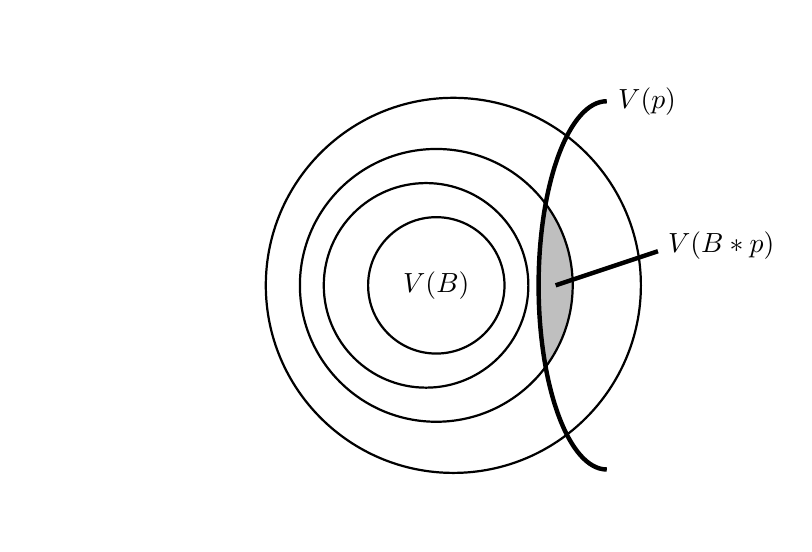
\begin{tikzpicture} [scale=\textwidth/14cm]

    \definecolor{lightgray}{gray}{0.75};
    
    % these coordinates guarantee the graph's total size
    \node at (-6,3.5) [draw=none,fill=none, above right] { }; \node at
    (3.5,-3.5) [draw=none,fill=none, above right] { };
    
    \begin{scope}
    \clip (0,0) circle (2.0); \fill[lightgray] (2.5,2.7) arc (90:270:1 and 2.7);
    \end{scope}
    
    %spheres
    \begin{scope} [thick]
    %inner sphere \draw (0,0) circle (0.5) node {$V(B)$}; 2nd sphere
    \draw (0,0) circle (1) node {$V(B)$};
    %3rd sphere
    \draw (-.15,0) circle (1.5);
    %4th sphere
    \draw (0,0) circle (2);
    %5th sphere
    \draw (.25,0) circle (2.75);
    \end{scope}
    
    %new information
    \begin{scope} [ultra thick] \draw (2.5,2.7) node [right] {$V(p)$} arc
    (90:180:1 and 2.7) node [above=0.5cm,right=1.5cm,fill=white] {$V(B*p)$} arc
    (180:270:1 and 2.7);
    
    %line leading to caption
    \draw (1.75,0) -- (3.25,0.5);
    \end{scope}
    
    \end{tikzpicture}
    \caption{A system of spheres centered on $V(B)$. The shaded region is $V(B*p)$. }
  \label{fig:boat1}
\end{figure}
Given a belief set $B$ and a system of spheres $\mathcal{S}$ centered on $V(B)$
we can define a revision operator by setting: $$B*p = T(\mathcal{S}(p)).$$ The
idea is this: when you revise on a sentence $p$ compatible with your previous
beliefs, then the strongest proposition you believe is $V(p) \cap V(B).$ If $p$
is incompatible with your beliefs, you fall back to $E\cap V(p),$ where $E$ is
the $p$-compatible proposition closest to your old belief $V(B)$. Thus, the
system of spheres $\mathcal{S}$ can be seen as a set of ``fallback positions''
for updating on incompatible propositions. See \autoref{fig:boat1}.

\citet{grove1988two} proves the following.
\begin{theorem}
Let $B$ be a belief set. For each system of spheres $\mathcal{S}$ centered on
$V(B),$ there is an operation $*$ satisfying the six basic and the two
supplementary revision postulates such that $B*p = T(\mathcal{S}(p)).$ Moreover,
for every revision operation $*$ satisfying the six basic and the two
supplementary revision postulates, there is a sphere system $\mathcal{S}$
centered on $V(B)$ such that $B*p=T(\mathcal{S}(p)).$ 
\end{theorem}
Finally, the sphere semantics gives a dramatic illustration of the critique that
AGM does not illuminate iterated belief change. A revision maps a set of spheres
$\mathcal{S}$ and a sentence $p$ to a {\em set of sentences}
$T(\mathcal{S}(p)).$ It does not output a new set of spheres centered on the new
belief state. That severely underdetermines the result of future revisions.   

\subsection{The Paradox of the Preface}

The models of full belief that we have seen so far require that beliefs be
consistent and closed under deductive consequence. While it is admitted that
this requirement is not psychologically realistic, or perhaps even feasible for
bounded agents, it is proffered as a normative principle that we should strive
to approximate. After all, consistency and closure are {\em necessary}
conditions for achieving the following two related ends: believing only true
sentences (consistency) and believing as many true sentences as possible without
risking error in any more possible worlds (closure). 

Nevertheless, the Paradox of the Preface,  due to \citet{makinson1965preface},
challenges even the {\em normativity} of deductive consistency. The story goes
like this. A famous theorist has just finished her latest book. As is customary
for such works, she includes a passage in the preface thanking her colleagues
and students for their help in editing and proofreading, but accepting sole
responsibility for the mistakes that inevitably remain. She seems to be saying
that, despite her best efforts, she believes that not everything that she asserts
in the book is true. Let $s_1, \ldots, s_n$ be the claims she asserts in the
book. Presumably, she believes each of the $s_i$ or else she would not have
asserted them. Yet in the preface she claims to believe
$\neg(s_1\wedge\ldots\wedge s_n),$ the claim that at least one of the $s_i$ is
false. The theorist seems to be behaving perfectly rationally, yet on this
reconstruction there is no way that she can be both consistent and deductively
closed.

It is tempting to say that inconsistency in the service of intellectual humility
is no sin. Yet this creates a further difficulty: surely some inconsistencies
are vicious and should be eliminated. Others, it seems, are virtuous and ought
to be tolerated. But how do we know which inconsistencies are which? If we point
out an inconsistency in someone's beliefs, we tend to think that they are under
some pressure to resolve it. But why can't everyone respond to such a challenge
by claiming that their inconsistency is a virtue? The Preface Paradox seems to
challenge the very normativity of logical consistency.

There are several ways to respond to this challenge. The first, and perhaps the
most common route, is to claim that belief is fundamentally a matter of degree.
The theorist merely has a high {\em degree} of belief in each of the statements
of her book. And there is nothing surprising about having a high degree of
belief in each of the $s_i$ but not in their conjunction. In fact, if the
structure of partial belief is probabilistic, this would emerge as a simple
consequence of the probability calculus: it is to be expected that the
probability of each of the $s_i$ exceeds the probability of their conjunction,
so long as the probability of the $s_i$ falls short of unity. This analysis also
entails something about the relationship between full and partial belief: it is
rationally admissible to fully believe statements that have a high, but not
maximal, degree of belief. These themes will be taken up in subsequent sections.

A second set of responses to the paradox calls our attention to the variety of
cognitive attitudes that are involved in the story. For example,
\citet{cohen1992essay} attributes many confusions and apparent paradoxes to the
erroneous conflation of two related cognitive attitudes: belief and {\em
acceptance}. Belief in $p$, according to Cohen, is a disposition to feel it true
that $p$, whenever attending to issues raised by the proposition that $p.$ This
disposition may or may not be reflected in speech and action, and is not under
direct volitional control. But to {\em accept} that $p$ is to adopt a policy of
deeming, positing, or postulating that $p$---i.e. of including it among one's
premises for deciding what to do or think in a particular context, whether or
not one feels it to be true. Acceptance is a volitional matter, and is sensitive
to our cognitive context.

Belief is sometimes not even a {\em prima facie} reason for acceptance: in
scientific contexts many of our most cherished beliefs are not accepted, as it
is our duty to subject them to criticism and not argue from them as premises.
Cohen claims that a person who accepts nothing that she believes is
intellectually paralyzed, but someone who accepts everything she believes is
recklessly uncritical. Furthermore, acceptance may sometimes promote belief, at
least in the long run, but often has no effect: for example, a defense lawyer
may accept that her client is innocent, but believe otherwise.  

Cohen claims that acceptance ought to be closed, at least under accepted
deductive consequences. Consistency is also, presumably, a norm of acceptance.
Belief, however, is different:
\begin{quote}
\ldots you are not intellectually pledged by a set of {\em beliefs}, however strong, to each deductive consequence of that set of beliefs, even if you recognize it to be such. That is because belief that $p$ is a disposition to feel that $p$, and feelings that arise in you \ldots through involuntary processes \ldots no more impose their logical consequences on you than do the electoral campaign posters that people stick on your walls without your consent. \citep[p. 31]{cohen1992essay}
\end{quote}

Armed with the distinction between belief and acceptance, we can attempt a
redescription of the preface paradox. In the context of her theoretical work,
the theorist accepts $s_1, \ldots, s_n$ and is bound to maintain consistency and
accept their (accepted) deductive consequences. In fact, she would be in
dereliction of her duty as theorist if she accepted the preface sentence in the
body of the book. However, the context of the preface is different: here it is
customary to drop the professional exigencies of the theorist and acknowledge
broader features of the author's cognitive life. She has fulfilled her duty as
theorist and done the utmost to accept only those claims that are justified by
her evidence and arguments. However, some of these conclusions may not yet be
attended with the inner glow of belief. Perhaps, if the work meets with no
devastating objections, she may eventually cease to believe the humble claim in
the preface. Thus the distinction between belief and acceptance explains why we
are not alarmed by the sentence in the context of the preface, but we would be
shocked if we saw it used as a premise in the body of the text. For a similar
resolution of the paradox, see Chapter 5 of \citet{stalnaker1984inquiry}.

It is easy to underestimate the consequences of accepting Cohen's arguments. For
one, we would have to reinterpret all of the theories of rational belief that we
have discussed as theories of rational acceptance. In fact, there may be no
theory of rational belief, but only psychological tricks and heuristics for
coming to believe, similar to those Pascal recommends for arriving at faith in
Christ. Longstanding dogmas about the relation between belief and knowledge
would have to be revisited. Moreover, excessive appeal to the distinction
threatens the unity and cohesiveness of our cognitive lives. For a discussion of
these kinds of objections see \citet{kvanvig2016intellectual}. For an overview
of the distinction between belief and acceptance, see \citet{weirich2004belief}.


  
\section{Structures for Partial Belief}
\subsection{Bayesianism}

Bayesianism, or subjective probability theory, is by far the dominant paradigm
for modeling partial belief. The literature on the subject is by now very large
and includes many approachable introductions. The summary provided here will, of
necessity, be rather brief. For an article-length introduction see
\citet{sep-formal-belief}, \citet{easwaran2011bayesA,easwaran2011bayesB}, or
\citet{weisberg2011varieties}. For a book-length introduction see
\citet{earman1992bayes} or \citet{howson2006scientific}. For an article-length
introduction to Bayesian models of rational action, see
\citet{sep-rationality-normative-utility}. For an approachable book-length
introduction to the theory of rational choice see \citet{resnik1987choices}. 

The heart of the Bayesian theory is roughly the following:
\begin{enumerate}
  \item There is a fundamental psychological attitude called {\em degree of
  belief} (sometimes called {\em confidence} or {\em credence}) that can be
  represented by numbers in the $[0,1]$ interval.
  \item The degrees of belief of rational agents satisfy the axioms of
  probability theory.
  \item The degrees of belief of rational agents are {\em updated} by some
  flavor of probabilistic conditioning.
\end{enumerate}
The first two principles are the synchronic requirements of Bayesian theory; the
third principle concerns diachronic updating behavior. Most Bayesians would also
agree to some version of the following principles, which link subjective
probabilities with deliberation and action:
\begin{enumerate}\setcounter{enumi}{3}
  \item Possible states of the world (sometimes {\em outcomes}) are assigned a
  {\em utility}: a positive or negative real number that reflects the
  desirability or undesirability of that outcome.
  \item Rational agents perform only those actions that maximize {\em expected}
  utility, which is calculated by weighing the utility of outcomes by their
  subjective probability.
\end{enumerate}

What makes Bayesianism so formidable is that, in addition to providing an
account of rational belief and its updating, it also provides an account of
rational action and deliberation. No other theory can claim a developed,
fine-grained account of all three of these aspects of belief. In the following
we will briefly spell out some of the technical details of the Bayesian picture.



\subsubsection{Probabilism}

In this section we flesh out the details of the synchronic component of the
Bayesian theory. For the purposes of this section we will take propositions to
be the objects of (partial) belief. It is also possible to take a syntactic
approach and assign degrees of belief to sentences in a formal language. For the
most part, nothing hinges on which approach we choose. For arguments in favor of
the syntactic approach, see \citet{weisberg2011varieties}. 

As usual, let $W$ be a set of possible worlds. Let $\mathcal{F}$ be a
$\sigma$-field over $W$.\footnote{Refer to \autoref{objects} if you need to
refresh yourself on the definition of a $\sigma$-field.} A {\em credence}
function $p$ assigns a degree of belief to every proposition in $\mathcal{F}$.
{\em Probabilism} requires that the credence function satisfies the axioms of
probability. For every $E,F \in \mathcal{F}$: 
\begin{itemize}
\item[] $p(E)$ is a positive, real number; \hfill (Positivity)
\item[] $p(W)=1$; \hfill (Unitarity)
\item[] if $E\cap F= \varnothing$, then $p(E\cup F)=p(E)+p(F)$. \hfill
(Additivity)
\end{itemize}
From these principles it is possible to derive several illuminating theorems.
For example, the degree of belief assigned to the contradictory proposition is
equal to zero. Furthermore, if $E$ entails $F,$ then $p(E)\leq p(F)$. Finally,
for any proposition $E\in\mathcal{F}$ we have that $0\leq p(E)\leq 1.$

In the standard axiomatization of probability theory due to
\citet{kolmogorov1950foundations}, additivity is strengthened to Countable
Additivity.
\begin{itemize}
\item[] If $E_1, E_2, \ldots$ are mutually
exclusive,\\$\phantom{M}$\hspace{1.5em} then $p(\bigcup_{i=1}^\infty E_i) =
\sum_{i=1}^\infty p(E_i)$. \hfill(Countable Additivity)
\end{itemize}
This requirement is not as innocent as it looks: it rules out the possibility
that any agent is indifferent over a countably infinite set of mutually
exclusive possibilities. \Citet{definetti1970theory, definetti1972probability}
famously argued that we ought to reject countable additivity since it is
conceivable that God could pick out a natural number ``at random'' and with
equal (zero) probability. For another example, suppose you assign $50\%$
credence to the proposition $\neg B$ that not all ravens that will ever be
observed are black. Let $\neg B_i$ be the proposition that the $i^\text{th}$
observed raven is the first non-black raven to appear. Then $\neg B =
\bigcup_{i=1}^\infty \neg B_i.$ Countable additivity entails that for all
$\epsilon>0$ there is a finite $n$ such that $p(\bigcup_{i=1}^n \neg B_i) = 1/2
-\epsilon.$ So you must be nearly certain that if all ravens are not black, the
first non-black raven will appear among the first $n$ ravens. The only way to
assign equal probability to all $\neg B_i$ is to violate countable additivity by
setting $p(\neg B_i)=0$ for all $i$. This solution has its own drawbacks. On all
standard models of Bayesian update it will be impossible to become convinced
that the $i^\text{th}$ raven is indeed non-black, even if you are looking at a
white one. For more on countable additivity, see Chapter 13 in
\citet{kelly1996logic}.

Now that we have defined probabilism, it is natural to ask how to justify it:
why {\em should} a rational agent's degrees of belief obey the probability
axioms? There are roughly two kinds of answers to this question current in the
Bayesian canon.

The traditional answer is that an agent that violates the axioms of probability
opens herself up to systems of bets that, although fair from the agent's
perspective, guarantee a sure loss. Answers of this flavor are called {\em Dutch
book} arguments and they require positing some connection between degrees of
belief and fair betting quotients. Some epistemologists find Dutch book
arguments to be unconvincing either because they disavow any tight connection
between degrees of belief and betting quotients, or they deny that any facts
about something so pragmatic as betting could have normative epistemic force.
These epistemologists tend to prefer {\em accuracy} arguments, which purport to
show that any agent violating the probability axioms will have beliefs which are
less accurate, or ``further from the truth,'' than agents that satisfy the
axioms. We will briefly review the traditional Dutch book-style arguments. For
the original articulation of the accuracy perspective see
\citet{joyce1998nonpragmatic}. For an article-length overview of accuracy-style
arguments see \citet{sep-epistemic-utility}. For a book-length treatment see
\citet{pettigrew2016accuracy}.  

Dutch book arguments require specifying some connection between degrees of
belief and fair betting quotients. For \citet{de1937prevision} the connection
was definitional: an agent's degree of belief in a proposition $A$ simply is her
fair odds ratio for a bet that pays $\$1$ if $A$ is true and nothing otherwise.
If you are willing to pay at most $\$.50$ for a bet that pays $\$1$ if $A$ is
true and nothing otherwise, then it must be that your degree of confidence in
$A$ is $50\%$. It is easy to see what is wrong with this kind of definition:
there may be factors other than the subject's degree of belief which affect her
fair betting quotient. She may be risk averse, or risk-loving; she may abhor
gambling, or love showing off. \citet{ramseytruth} avoids some of these problems
by pricing bets in utility, rather than money, and appealing to the existence of
an ``ethically neutral'' proposition that is considered equally likely to be
true and false. For more on the connection between degrees of belief and betting
ratios see \citet{eriksson2007degrees}.

Supposing that a suitable connection between degrees of belief and fair betting
quotients exists, it is possible to construct a ``Dutch book'' against an agent
violating the axioms of probability. To get such an argument going we suppose
that if the agent's degree of belief in $A$ is $p(A),$ then she considers fair a
bet that costs $\$ p(A)\cdot Y$ and pays $\$Y$ if $A$ is true and $\$0$
otherwise. Note that we allow $Y$ to take positive and negative values. This
means that the agent is willing to assume the role of the bookie and sell a bet
that ``costs'' $-\$ p(A)\cdot Y$ and ``pays'' $-\$Y$ if $A$ is true and $\$0$
otherwise. Now suppose that such an agent violates finite additivity. One way
this may happen is if for $A,B$ such that $A\cap B = \varnothing$, we have that
$p(A\cup B) > p(A) + p(B).$ Then, the agent considers fair
\begin{enumerate}
\item a bet that costs $-\$p(A)$ and pays $-\$ 1$ if $A$ is true and $\$ 0$
otherwise; 
\item a bet that costs $-\$p(B)$ and pays $-\$ 1$ if $B$ is true and $\$ 0$
otherwise; 
\item a bet that costs $\$p(A\cup B)$ and pays $\$1$ if $A\cup B$ is true and
$\$0$ otherwise.
\end{enumerate}
There are three possible scenarios: either $A$ and $B$ are both false or exactly
one of them is true. The reader should confirm that in any of these scenarios
the agent is left with exactly $ \$p(A) + \$p(B) - \$p(A\cup B) < 0.$ By
reversing which bets the agent buys and sells, we can construct a Dutch book
against an agent that violates additivity by having $p(A\cup B) < p(A) + p(B).$
Similar strategies work to construct Dutch books against agents that violate
Positivity, Unitarity, and Countable Additivity. Furthermore, it is possible to
show that if your degrees of belief validate the probability axioms, then no
Dutch book can be made against you \citep{kemeny1955fair}. For more on Dutch
book arguments see Section 3.3 in \citet{sep-probability-interpret}.

\subsubsection{Updating by Conditioning}

We have discussed the synchronic content of the Bayesian theory, but we still
need to talk about how degrees of belief are updated upon receiving new
information. There are two standard models of partial belief update: strict
conditionalization and Jeffrey conditionalization. Strict conditionalization
assumes that the information received acquires the maximal degree of belief.
Jeffrey conditionalization allows for the situation in which no proposition is
upgraded to full certainty when new information is acquired.

For all propositions $A,B\in \mathcal{F}$ such that $p(A)>0$, the conditional
probability of $B$ given $A$ is defined as: $$p(B \given A) := \frac{p(A\cap
B)}{p(A)}.$$ Conditionalization by $A$ restricts all possibilities to those
compatible with $A$ and then renormalizes by the probability of $A$ to ensure
that unitarity holds. By far the most standard modeling of partial belief update
holds that degrees of belief ought to be updated by conditionalization. In other
words, if $p_t$ is your credence function at time $t$ and $A$ is a proposition
expressing the total new information acquired by $t'>t,$ then $p_{t'}$ ought to
equal $p_t(\cdot \given A),$ whenever $p_t(A)>0.$

What if new information does not render any proposition certain, but merely
changes the subjective probability of some propositions?
\citet{jeffrey1983logic} proposes the following update rule. Suppose that $p_t$
is your credence function at time $t$. Suppose that the total evidence that
comes in by time $t'$ updates your degrees of belief in partition
$\{A_i\}_{1\leq i \leq n}$ (and in no finer partition) setting each respectively
to $a_i$ with $\sum_i a_i = 1.$ Then your new credence function $p_{t'}$ ought
to be $\sum_i p(\cdot \given A_i) a_i.$ 

Why should a rational agent update by strict or Jeffrey conditionalization?
Dutch-book style arguments for strict conditionalization are given in
\citet{teller1973conditionalization} and \citet{lewis1999why} and extended to
Jeffrey conditionalization in \citet{armendt1980isthere}. For more see
\citet{skyrms2006diachronic}. For an accuracy-style argument in favor of strict
conditionalization and against Jeffrey conditionalization, see
\citet{leitgeb2010objective}.

For our purposes it is important to point out that conditional probability is
always a lower bound for the probability of the material conditional. In other
words, for all $E,H\in \mathcal{F},$ $$p(H \given E)\leq p(E\rightarrow H),$$
whenever $p(E)>0$. We can see this as a quantitative version of the qualitative
principle of Conditionalization we discussed in \autoref{nonmonprinciples}:
however confident a Bayesian agent becomes in $H$ after updating on $E,$ she
must have been at least as confident that $H$ is a material consequence of $E$.
\citet{popper1983proof} took this observation to be ``completely devastating to
the inductive interpretation of the calculus of probability.'' For the history of
the Popper-Miller debate see Chapter 4 in \citet{earman1992bayes}. A similar
property can be demonstrated for Jeffrey conditioning
\citep{genin2017howinductive}.

Both strict and Jeffrey conditionalization are defined in terms of conditional
probability. The probability of $B$ conditional on $A$ is standardly defined as
the ratio of the unconditional probabilities $p(A\cap B)$ and $p(A)$. Clearly,
this ratio is undefined when $p(A)=0$. Some theorists would like conditional
probability to be defined even when conditioning on propositions of probability
zero. The standard approach in mathematical statistics, due to
\citet{kolmogorov1950foundations}, is via the {\em conditional expectation}. On
that approach, conditional probability remains dependent on unconditional
probability. An alternative approach, adopted by \citet{popper1955probability}
and \citet{renyi1955newsystem}, takes conditional probability as a primitive,
rather than a derivative, notion. For a defense of the conditional expectation,
see \citet{gyenis2017conditioning}. For an introduction to primitive conditional
probabilities, see Easwaran (\citethisvolume{thisvolume:easwaran}). For a critique of the standard
notion of conditional probability, see \citet{hajek2003what}. 


\subsubsection{Deliberation and Action}

One of the signal advantages of the Bayesian model of partial belief is that it
is ready-made to plug into a prominent model of practical deliberation. Decision
theory, or rational choice theory, is too large and sprawling a subject to be
effectively covered here, although it will be presented in cursory outline. For
an excellent introduction, see \citet{sep-rationality-normative-utility} or Thoma
(\citethisvolume{thisvolume:thoma}). For our purposes, it is enough to note that a
well-developed theory exists and that no comparable theory exists for
alternative models of belief.\footnote{However, recent work such as
\citet{lin2013foundations} and \citet{spohn2017knightian, spohn2019defeasible}
may remedy that inadequacy in the case of qualitative belief.}

Suppose you would like to make a six egg omelet. You've broken $5$ fresh eggs
into a mixing bowl. Rooting around your fridge, you find a loose egg of
uncertain provenance. If you are feeling lucky you can break the suspect egg
directly into the mixing bowl; if you are wary of the egg, you might break it
into a saucer first and incur more dishwashing.

There are four essential ingredients to this sort of decision-theoretic
situation. There are {\em outcomes}, over which we have defined {\em utilities}
measuring the desirability of the outcome. In the case of the omelet the
outcomes are a ruined omelet or a $5$--$6$ egg omelet, with or without extra
washing. There are {\em states}---usually unknown to and out of the control of
the actor---which influence the outcome of the decision. In our case the states
are exhausted by the possible states of the suspect egg: either good or rotten.
Finally, there are {\em acts} which are under the control of the decision maker.
In our case the acts include breaking the egg into the bowl or the saucer. Of
course there are other conceivable acts: you might throw the suspect egg away
and make do with a $5$-egg omelet; you might even flip a coin to decide what to
do. We omit these for the sake of simplicity. These four elements are usually
summarized in a payoff table (see \autoref{omelet}).
\begin{table}
\centering
\begin{tabular}{ccc}%\hline
    &\multicolumn{2}{ c } {\textbf{States}} \\%\hline
    \cline{2-3}
&Good\phantom{: 50\%}&Rotten\phantom{: 50\%}\\\hline
\multicolumn{1}{ c } {\textbf{Acts}}&\multicolumn{2}{ c }{\textbf{Outcomes}}
\\\hline\hline  
\multicolumn{1}{l}{\textsc{Break into Bowl}\phantom{(A1)}}&$6$-Egg Omelet&No
Omelet\\
\multicolumn{1}{c}{}&{$+10$}&\textcolor{black}{{$0$}}\\
\multicolumn{1}{l}{\textsc{Break into Saucer}\phantom{(A1)}}&$6$-Egg
Omelet,&$5$-Egg Omelet,\\
\multicolumn{1}{c}{}&extra washing&extra washing\\
\multicolumn{1}{c}{}&\textcolor{black}{{$+8$}}&\textcolor{black}{{$+4$}}\\\hline
\end{tabular}
\caption{A payoff table for the morning chef}\label{omelet}
\end{table}
To fit this into the framework of partial belief we assume that the set of acts
$A_1, A_2, \ldots, A_n$ partition $W$. We also assume the set of states $S_1,
S_2, \ldots, S_m$ partition $W$. We assume that the credence function assigns a
probability to every outcome. We assume that acts and states are logically
independent, so that no state rules out the performance of any act. Finally, we
assume that given a state of the world $S_j$ and an act $A_i$ there is exactly
one outcome $O_{ij}$, which is assigned a utility $U(O_{ij})$. The ultimate
counsel of rational choice theory is that agents ought to perform only those
acts that maximize {\em expected} utility. The expected utility of an act is
defined as:
$$ EU(A_i) = \sum_{j=1}^m p_{A_i}(S_j)U(O_{ij}),$$ where $p_{A_i}(S_j)$ is
roughly how likely the agent considers $S_j$ given that she has performed act
$A_i$. Difficulties about how this quantity should be defined give rise to the
schism between evidential and causal decision theory (see Section 3.3 in
Thoma, \citethisvolume{thisvolume:thoma}). However, in many situations, including the dilemma
of the omelet, the act chosen does not affect the probabilities with which
states obtain. This is called ``act-state independence'' in the jargon of
rational choice theory. In cases of act-state independence there is broad
consensus that $p_{A_i}(S_j)$ should be equal to the unconditional degree of
belief $p(S_j)$.

Central to the literature on decision theory are a number of {\em representation
theorems} showing that every agent with qualitative preferences satisfying a set
of rationality postulates can be represented as an expected utility maximizer
\citep{vonneumann1944theory, savage1954foundations}. These axioms are
controversial, and are subject to intuitive counterexamples.
\citet{allais1953lecomportement} and \citet{ellsberg1961risk} give examples in
which seemingly rational agents violate the rationality postulates and therefore
cannot, even in principle, be represented as expected utility maximizers. For
more on this subject, see Sections 2 and 3 in
\citet{sep-rationality-normative-utility}.

\subsubsection{Modifications and Alternatives}

Dissatisfaction with various aspects of the Bayesian theory has spawned a number
of formal projects. Many epistemologists reject the notion that rational agents
must have {\em precise} credences in every proposition that they can entertain;
instead they claim that rational agents may have {\em imprecise} credences
representable by {\em intervals} of real numbers. For an introduction to
imprecise probability, see Mahtani (\citethisvolume{thisvolume:mahtani}). The theory of
Dempster-Shafer belief functions \citep{dempster1968generalization,
shafer1976mathematical} rejects the tight connection between degrees of belief
and fair betting ratios. Fair betting ratios ought indeed satisfy the axioms of
probability, but degrees of belief need not. Nevertheless, it should be possible
to calculate fair betting ratios from degrees of belief when these are
necessary. For this purpose, degrees of belief may satisfy a weaker set of
axioms than those of the probability calculus. For an introduction to
Dempster-Shafer belief functions see Section 3.1 in \citet{sep-formal-belief}.

Many epistemologists have held that degrees of belief are not so definitely
comparable as suggested by the probabilistic analysis.
\citet{keynes1921treatise} famously proposes that degrees of belief may enjoy
only an {\em ordinal} structure, which admits of qualitative, but not
quantitative, comparison. Keynes even suggests that the strength of some pairs
of partial beliefs cannot be compared at all. \citet{koopman1940axioms} and
\citet{fine1973theories} pursue Keynes' suggestions, developing axiomatic
theories of qualitative probability. See Konek (\citethisvolume{thisvolume:konek}) for an
introduction to qualitative probability comparisons. 

\subsection{Ranking Theory}
\label{rankingtheory}

\Citet{cohen1977probable, cohen1980some} distinguishes between two rival
probabilistic traditions. Pascalian probability finds its latest expression in
contemporary Bayesianism. But Cohen traces a rival tradition back to Francis
Bacon. Roughly, these two can be distinguished by the {\em scale} they select
for the strength of belief. On the Pascalian scale a degree of belief of zero in
some proposition implies maximal conviction in its negation. On the Baconian
scale, a degree of belief of zero implies no conviction in either the
proposition or its negation. Thus, the Pascalian scale runs from ``disproof to
proof'' whereas the Baconian runs from ``no evidence, or non-proof to proof''
\citep[p. 224]{cohen1980some}.  \citet{cohen1977probable} argues that despite
the conspicuous successes of Pascalian probability, the Baconian scale is more
appropriate in other settings, including legal proceedings.

{\em Ranking theory}, first developed in \citet{spohn1988ordinal}, is a
sophisticated contemporary theory of Baconian probability. For an article-length
introduction to ranking theory see Huber (\citeyearhyper{huber2013ranking}; 
\citethisvolume{thisvolume:huber}).
For an extensive book-length treatment, with applications to many subjects in
epistemology and philosophy of science, see \citet{spohn2012laws}. We mention
some of its basic features, as it provides a useful counterpoint to the models
of belief we have already discussed.

As before, let $W$ be a set of possible worlds. Let $\mathcal{F}$ be an algebra
over $W$.\footnote{Refer to \autoref{objects} if you need to refresh yourself on
the definition of an algebra} A function $\beta: \mathcal{F} \rightarrow
\mathbb{N} \cup \{\infty\}$ from $\mathcal{F}$ into the set of natural numbers
$\mathbb{N}$ extended by $\infty$, is a {\em positive ranking function} on
$\mathcal{F}$ just in case for any $A,B\in\mathcal{F}$: 
\begin{itemize}
\item[] $\beta(\varnothing)=0;$ \hfill(Consistency)
\item[] $\beta(W)=\infty;$ \hfill(Infinitivity)
\item[] $\beta(A\cap B)=\min \{ \beta(A), \beta(B)\}.$ \hfill(Minimitivity)
\end{itemize}
A positive ranking function expresses degrees of belief. If $\beta(A)>0$, then
we may say that $A$ is (fully) believed and $\neg A$ is disbelieved. If
$\beta(A)=0$ then $A$ is not believed and $\neg A$ may not be believed either.
Thus, ranking theory can be seen as satisfying the ``Lockean thesis,'' the
intuitive proposal that a degree of belief above some threshold is necessary and
sufficient for full belief (see \autoref{lockeanthreshold}). Note however that
nothing in ranking theory requires us to say that the threshold is exactly zero:
we could have chosen any positive number $n$. 

Let $\beta$ be a positive ranking function and $A\in \mathcal{F}$ with
$\beta(\neg A) < \infty.$ Then for any $B\in\mathcal{F}$ the {\em conditional
positive rank of $B$ given $A$} is defined as $$ \beta(B \given A) = \beta(\neg
A \cup B) - \beta(\neg A).$$ The function $\beta_A : B \mapsto \beta(B \given
A)$ is called the {\em conditionalization of $\beta$ by $A$} and is itself a
positive ranking function. This definition is used to articulate an update rule
for ranking theory: if $\beta$ is your positive ranking function at time $t$ and
between $t$ and $t'$ you become certain of $E\in\mathcal{F}$ and no logically
stronger proposition, then $\beta_E$ should be your new ranking function at time
$t'.$ \citet{spohn1988ordinal} also defines ranking-theoretic analogues of
Jeffrey conditioning.

It is clear from the definition of conditioning that, as in the Bayesian case,
the rank of the material conditional is a lower bound for the conditional rank:
$\beta(A\rightarrow B) \leq \beta(B \given A).$ It also satisfies a version of
Rational Monotony: if $\beta(\neg A)=0$ and $\beta(B)>0,$ then $\beta(B \given
A)>0.$\footnote{Rational Monotony is not satisfied if we set the threshold for
full belief at some number greater than zero.} Therefore, ranking-theoretic
update satisfies the ``spirit'' of AGM update. Note however, that ranking theory
has no trouble with iterated belief revision: a revision takes as input a
ranking function and an evidential proposition and outputs a new ranking
function.

Ranking theory lies somewhat awkwardly between a theory of full and partial
belief. On the one hand, all propositions of positive rank are fully believed.
On the other hand, the rank of a proposition measures something about the
strength of that belief. But how should we interpret these ranks?
Huber (\citethisvolume{thisvolume:huber}) investigates the relation between ranking-theoretic
degrees of belief, and AGM-style degrees of entrenchment. The {\em degree of
entrenchment} for a proposition $A$ is defined as the number of independent and
reliable information sources testifying {\em against} $A$ that it requires for
the agent to give up full belief in $A$. Degrees of entrenchment may be used to
{\em measure} ranking-theoretic degrees of belief; alternatively, it is possible
to {\em identify} ranking-theoretic degrees of belief with degrees of
entrenchment. \citet{huber2019belief} proves that if an agent defines her full
beliefs from an entrenchment function, her beliefs will be consistent and
deductively closed iff the entrenchment function is a ranking function.

One of the advantages of ranking theory over AGM is that it allows {\em reasons}
to be defined \citep{spohn2012laws}. Say that {\em $A$ is a reason for $B$} with
respect to the positive ranking function $\beta$ iff $\beta(B \given A)>\beta(B
\given \neg A).$ Say that an agent {\em has $A$ as a reason for $B$} iff $A$ is
a reason for $B$ according to her positive ranking function $\beta$ and
$\beta(A)>0$. Note that it is not possible to make such a definition in the AGM
theory since the conditional degree of entrenchment is not defined. Thus ranking
theory may provide an answer to Pollock's criticism of belief revision by
allowing various kinds of defeat of reasons to be represented \citep[Section
11.5]{spohn2012laws}.  


\section{Eliminationisms}

There are those who deny that there are any interesting principles bridging full
and partial belief. Theorists of this persuasion often want either to eliminate
one of these attitudes or reduce it to a special case of the other.
\citet{jeffrey1970} suggests that talk of full belief is vestigial and will be
entirely superseded by talk of partial belief and utility:
\begin{quote}
\ldots  nor am I disturbed by the fact that our ordinary notion of {\em belief}
is only vestigially present in the notion of degree of belief. I am inclined to
think Ramsey sucked the marrow out of the ordinary notion, and used it to
nourish a more adequate view. But maybe there is more there, of value. I hope
so. Show me; I have not seen it at all clearly, but it may be there for all that
(p. 172). 
\end{quote}
Theorists such as \citet{kaplan1996decision} also suggests that talk of full
belief is superfluous once the mechanisms of Bayesian decision theory are in
place. After all, only partial beliefs (or {\em confidence} in Kaplan's
terminology) and utilities play any role in the Bayesian framework of rational
deliberation, whereas full belief need not be mentioned at all. Those committed
to full beliefs have the burden of showing what difference they make to our
lives:
\begin{quote}
Making the case that talk of investing confidence leaves out something
important---something we have in mind when we talk of belief---is going to
require honest toil. One has to say \ldots exactly how an account of rational
human activity will be the poorer if it has no recourse to talk of belief. In
short, one has to meet {\em the Bayesian Challenge}. (p. 100)
\end{quote}
\citet{stalnaker1984inquiry} is much more sympathetic to a qualitative notion of
belief (or acceptance) but acknowledges the force of the Bayesian Challenge.
\begin{quote}
Bayesian decision theory gives a complete account of how probability values
\ldots ought to guide behavior \ldots So what could be the point of selecting an
interval near the top of the probability scale and conferring on the
propositions whose probability falls in that interval the honorific title
``accepted''? Unless acceptance \ldots makes a difference to how the agent
behaves, or ought to behave it is difficult to see how the concept of acceptance
can have the interest and importance for inquiry that it seems to have. (p. 91)
\end{quote}
It is true that there is no canonical qualitative analogue to the Bayesian
theory of practical deliberation. However, the fact that it is the theorist of
full belief that feels the challenge, and not {\em vice versa}, may be an
accident of history: if a qualitative theory of practical deliberation had been
developed first, the shoe would now be on the other foot. The situation would be
even more severe if qualitative decision making, which we seem to implement as a
matter of course, were less cognitively demanding than its Bayesian counterpart.
Of course, this anticipates a robust  theory of rational qualitative
deliberation that is not immediately forthcoming. However, recent work such as
\citet{lin2013foundations} and \citet{spohn2017knightian, spohn2019defeasible}
may remedy that inadequacy. For example, \citet{lin2013foundations} proves a
Savage-style representation theorem characterizing the relationship between full
beliefs, desires over possible outcomes, and preferences over acts. By
developing a theory of rational action in terms of qualitative belief, Lin
demonstrates how one might answer the Bayesian challenge. 

On the other hand there are partisans of full belief that are deeply skeptical
about partial beliefs.\footnote{See \citet{harman1986change},
\citet{pollock2006thinking}, \citet{moon2017beliefs}, and
\citet{horgan2017troubles}. See also the ``bad cop'' in \citet{hajek2017tale}.}
Many of these object that partial beliefs have no psychological reality and
would be too difficult to reason with if they did. \citet{horgan2017troubles}
goes so far as to say that typically ``there is no such psychological state as
the agent's credence in $p$'' and that Bayesian epistemology is ``like alchemy
and phlogiston theory: it is not about any real phenomena, and thus it also is
not about any genuine norms that govern real phenomena'' (p. 7).
\citet{harman1986change} argues that we have very few explicit partial beliefs.
A theory of reasoning, according to Harman, can concern only explicit attitudes,
since these are the only ones that can figure in a reasoning process. Therefore,
Bayesian epistemology, while perhaps an account of dispositions to act, is not a
guide to reasoning. Nevertheless, partial beliefs may be implicit in our system
of full beliefs in that they can be reconstructed from our dispositions to
revise them.
\begin{quote}
How should we account for the varying strengths of explicit beliefs? I am
inclined to suppose that these varying strengths are implicit in a system of
beliefs one accepts in a yes/no fashion. My guess is that they are to be
explained as a kind of epiphenomenon resulting from the operation of rules of
revision. For example, it may be that $P$ is believed more strongly than $Q$ if
it would be harder to stop believing $P$ than to stop believing $Q$, perhaps
because it would require more of a revision of one's view\ldots \citep[p.
22]{harman1986change}
\end{quote}
On this picture, almost all of our explicit beliefs are qualitative. Partial
beliefs are not graded {\em belief attitudes} toward propositions, but rather
dispositions to revise our {\em full} beliefs. The correct theory of partial
belief, according to Harman, has more to do with entrenchment orders (see
\autoref{entrenchment}) or ranking-theoretic degrees of belief (see
\autoref{rankingtheory}) than with probabilities. Other apparently partial
belief attitudes are explained as full beliefs {\em about} objective
probabilities. So, in the case of a fair lottery with ten thousand tickets, the
agent does not believe to a {\em high degree} that the $n^\text{th}$ ticket will
not win, but rather fully believes that it is objectively improbable that it
will win.

\citet{frankish2009partial} objects that Harman's view requires that an agent
have a full belief in any proposition that we have a degree of belief in: ``And
this is surely wrong. I have some degree of confidence (less than $50\%$) in the
proposition that it will rain tomorrow, but I do not believe flat-out that it
will rain---not, at least, by the everyday standards for flat-out belief'' (p.
4). Harman might reply that Frankish merely has a full belief in the objective
probability of rain tomorrow. Frankish claims that this escape route is closed
to Harman because single events ``do not have objective probabilities,'' but
this matter is hardly settled.

\citet{staffel2013can} gives an example in which a proposition with a higher
degree of belief is apparently less entrenched than one with a lower degree of
belief. Suppose that you will draw a sequence of two million marbles from a big
jar full of red and black marbles. You do not know what proportion of the
marbles are red. Consider the following cases.
\begin{description}
\item[Scenario 1] You have drawn twenty marbles, $19$ black and one red. Your
degree of belief that the last marble you will draw is black is $.95$. 
\item[Scenario 2] You have drawn a million marbles, $900,000$ of which have
been black. Your degree of belief that the last marble you will draw is black is
$19/20=.90$. 
\end{description}
Staffel argues that your degree of belief in the first case is higher than in
the second, but much more entrenched in the second than in the first. Therefore,
degree of belief cannot be reduced to degree of entrenchment. Nevertheless, the
same gambit is open to Harman in the case of the marbles---he can claim that in
both scenarios you merely have a full belief in a proposition about objective
chance. See \citet{staffel2013can} for a much more extensive engagement with
\citet{harman1986change}. 



\section{Bridge Principles for Full and Partial Belief}\label{genin-sec-6}

Anyone who allows for the existence of both full and partial belief inherits a
thorny problem: how are full beliefs related to partial beliefs? That seemingly
innocent question leads to a treacherous search for {\em bridge principles}
connecting a rational agent's partial beliefs with her full beliefs. Theorists
engaged in the search for bridge principles usually take for granted some set of
rationality principles governing full belief and its revision e.g. AGM theory,
or a rival system of non-monotonic reasoning. Theorists usually also take for
granted that partial belief ought to be representable by probability functions
obeying some flavor of Bayesian rationality. The challenge is to propose
additional rationality postulates governing how a rational agent's partial
beliefs cohere with her full beliefs. In this section, we will for the most part
accept received wisdom and assume that orthodox Bayesianism is the correct model
of partial belief and its updating. We will be more open-minded about the
modeling of full belief and its rational revision. 

In this section, we will once again take propositions to be the objects of
belief. In the background, there will be a (usually finite) set $W$ of possible
worlds. As before, the reader is invited to think of $W$ as a set of
coarse-grained, mutually exclusive, possible ways the actual world might be. The
actual world is assumed to instantiate one of these coarse-grained
possibilities. We write $\Bel$ to denote the set of {\em propositions} that the
agent believes and use $\Bel(A)$ as shorthand for $A\in \Bel$. We will also
require some notation for qualitative propositional belief change. For all
$E\subseteq W$, write $\Bel_E$ for the set of propositions the agent would
believe upon learning $E$ and no stronger proposition. We will also write
$\Bel(A \given E)$ as shorthand for $A\in \Bel_E.$ By convention, $\Bel=
\Bel_W.$ If $\mathcal{F}$ is a set of propositions, we let $\cb_{\mathcal{F}}$
be the set $\{ \Bel_E : E \in \mathcal{F} \}.$ The set $\cb_{\mathcal{F}}$
represents an agent's {\em dispositions} to update her qualitative beliefs given
information from $\mathcal{F}$. 

The following normative constraint on the set of full beliefs $\Bel$ plays a
large role in what follows.
\begin{itemize}
\item[] For all propositions $A,B \subseteq W$: \hfill(Deductive Cogency)
  \begin{enumerate}
  \item $\Bel(W);$
  \item not $\Bel(\varnothing);$
  \item if $\Bel(A)$ and $A\subseteq B,$ then $\Bel(B);$
  \item if $\Bel(A)$ and $\Bel(B)$ then $\Bel(A\cap B).$
  \end{enumerate}
\end{itemize}
The first two clauses say that the agent believes the true world to be among the
worlds in $W$ and that she does not believe the empty set to contain the true
world. The third clause says that belief is closed under single-premise
entailment, i.e. if the agent believes $A$ and $A$ logically entails $B$, then
she believes $B$. The final clause says that the agent's beliefs are closed
under conjunction, i.e. if she believes $A$ and she believes $B$, then she
believes $A\cap B.$ Together, clauses 3 and 4 say that the agent's beliefs are
closed under entailment by finitely many premises. When $W$ is finite, the set
$\cb$ must be finite as well, implying that Deductive Cogency is equivalent to
the following formulation:
\begin{itemize}
\item[] $\Bel$ is consistent and $\Bel(B)$ iff $\cap \Bel \subseteq B.$ \hfill
(Deductive Cogency)
\end{itemize}
In other words, Deductive Cogency means that there is a single, non-empty
proposition, which is the logically strongest proposition that the agent
believes,  entailing all her other beliefs. When the two formulations of
Deductive Cogency come apart, we will always mean the latter one.% Note that
Deductive Cogency only mentions the set of full beliefs $\Bel,$ and is therefore
not a bridge principle at all. Bridge principles are expressed as constraints
holding for pairs $\langle \Bel,p \rangle$.   

All of the rationality norms that we have seen for updating qualitative beliefs
have propositional analogues.  The following are propositional analogues for the
six basic AGM principles. Here $E,F$ are arbitrary subsets of $W$.
\begin{itemize}
\item[] $\Bel_E=\Cn(\Bel_E)$. \hfill(Closure)
\item[] $E\in \Bel_E$. \hfill(Success)
\item[] $\Bel_E \subseteq \Cn(\Bel \cup \{ E\})$. \hfill(Inclusion)
\item[] If $\neg E \notin \Cn(\Bel)$ then $\Bel \subseteq \Bel_E$.
\hfill(Preservation)
\item[] $\Bel_E$ is consistent if $E\neq \varnothing$. \hfill(Consistency)
\item[] If $E\equiv F,$ then $\Bel_E = \Bel_F$. \hfill(Extensionality)
\item[] $\Bel_{E\cap F} \subseteq \Cn(\Bel_{E} \cup \{F\})$. \hfill(Conjunctive
inclusion)
\item[] If $\neg F \notin \Cn(\Bel_E)$, then\\$\phantom{M}$\hspace{1.5em}
$\Cn(B_E \cup \{F\}) \subseteq B_{E\cap F}$. \hfill(Conjunctive preservation)
\end{itemize}
Supposing that for all $E\subseteq W$, $\cb_E$ satisfies Deductive Cogency, the
first six postulates reduce to the following three, for arbitrary $E\subseteq
W$.
\begin{itemize}
\item[] $\cap \Bel_E \subseteq E$. \hfill(Success)
\item[] $\cap \Bel \cap E \subseteq \cap \Bel_{E}$. \hfill(Inclusion)
\item[] If $\cap \Bel \nsubseteq \neg E,$ then $\cap \Bel_{E} \subseteq \cap
\Bel \cap E.$ \hfill(Preservation)
\end{itemize}
Together, Inclusion and Preservation say that whenever information $E$ is
consistent with  current belief $\cap \Bel,$ $$\cap \Bel_E = \cap \Bel \cap E.$$
If $\mathcal{F}$ is a collection of propositions and for all $E\in \mathcal{F},$
the belief sets $\cb,\cb_E$ satisfy the AGM principles, we say that
$\cb_{\mathcal{F}},$ the agent's disposition to update her qualitative beliefs
given information from $\mathcal{F}$, satisfies the basic AGM principles.

We will use $p(\cdot)$ to denote the probability function representing the
agent's partial beliefs. Of course, $p(\cdot)$ is defined on a $\sigma$-algebra
of subsets of $W$. In the usual case, when $W$ is finite, we can take the
$\powerset(W)$ to be the relevant $\sigma$-algebra. To update partial belief, we
adopt the standard probabilistic modeling. For $E\subseteq W$ such that
$p(E)>0,$ $p(\cdot \given E)$ is the partial belief function resulting from
learning $E.$ We will sometimes use $p_E$ as a shorthand for $p(\cdot \given
E)$. Almost always, partial belief is updated via conditioning: $$p(A \given E)
= \frac{p(A\cap E)}{p(E)}, \text{ whenever } p(E)>0.$$ Let $\mathcal{F}_p^+$ be
the set of propositions with positive probability according to $p$, i.e $\{ A
\subseteq W : p(A)>0\}.$
  \subsection{Belief as Extremal Probability}
The first bridge principle that suggests itself is that full belief is just the
maximum degree of partial belief. Expressed probabilistically, it says that at
all times a rational agent's beliefs and partial beliefs can be represented by a
pair $\langle \Bel,p \rangle$ satisfying:

\begin{itemize}
\item[] $\Bel(A) \text{ iff } p(A)=1.$ \hfill (Extremal Probability)
\end{itemize}
\citet{roorda1995wolfman} calls this the {\em received view} of how full and
partial belief ought to interact. \citet{gardenfors1986dynamics} is a
representative of this view, as are \citet{van1995fine} and
\citet{arlo1999qualitative}, although the latter two accept a slightly
non-standard probabilistic modeling for partial belief. For fans of Deductive
Cogency, the following observations  ought to count in favor of the received
view.
\begin{theorem}
If $\langle \Bel, p \rangle$ satisfy extremal probability, then $\Bel$ is
deductively cogent.
  \end{theorem}
\citet{gardenfors1986dynamics} proves the following. 
\begin{theorem}
   Suppose that $\langle \cb_E, p_E \rangle$ satisfy extremal probability for
   all $E\in \mathcal{F}_p^+.$  Then $\cb_{\mathcal{F}_p^+}$  satisfies the AGM
   postulates. 
\end{theorem}
In other words: if an agent's partial beliefs validate the probability axioms,
she updates by Bayesian conditioning and fully believes all and only those
propositions with extremal probability, her qualitative update behavior will
satisfy all the AGM postulates (at least whenever Bayesian conditioning is
defined). Readers who take the AGM revision postulates to be a {\em sine qua
non} of rational belief update will take this to be good news for the received
view. 

\citet{roorda1995wolfman} makes three criticisms of the received view. Consider
the following three propositions.
\begin{enumerate}
\item Millard Fillmore was the 13th President of the United States;
\item Millard Fillmore was a U.S. President;
\item Millard Fillmore either was or was not a U.S. President. 
\end{enumerate}
Of course, I am not as confident that Fillmore was the $13^\text{th}$ president
as I am in the truth of the tautology expressed in (3). Yet there does not seem
to be anything wrong with saying that I fully believe each of (1), (2), and (3).
However, if extremal probability is right, it is irrational to fully believe
each of (1), (2), and (3) and not assign them all the same degree of belief.

Roorda's second objection appeals to the standard connection between degrees of
belief and practical decision making. Suppose I fully believe (1). According to
the standard interpretation of degrees of belief in terms of betting quotients,
I ought to be accept a bet that pays out a dollar if (1) is true, and costs me a
million dollars if (1) is false. In fact, if I truly assign unit probability to
(1), I ought to accept nearly any stakes whatsoever that guarantee some positive
payout if (1) is true. Yet it seems perfectly rational to fully believe (1) and
refrain from accepting such a bet. If we accept Bayesian decision theory,
extremal probability seems to commit me to all sorts of weird and seemingly
irrational betting behavior.

Roorda's final challenge to extremal probability appeals to {\em corrigibility},
according to which it is reasonable to believe that at least some of my beliefs
may need to be abandoned in light of new information. However, if partial
beliefs are updated via Bayesian conditioning, I can never cease to believe any
of my full beliefs since if $p(A)=1$ it follows that $p(A \given E)=1$ for all
$E$ such that $p(E)>0$. If we believe in Bayesian conditioning, extremal
probability seems to entail that I cannot revise any of my full beliefs in light
of new information.% Most theorists working in the area take these three
objections to be decisive against extremal probability. 

\subsection{The Lockean Threshold}
\label{lockeanthreshold}
The natural response to the difficulties with the received view is to retreat
from full certainty. Perhaps full belief corresponds to partial belief above
some {\em threshold} falling short of certainty. \citet{foley1993working} dubbed
this view the {\em Lockean thesis}, after some apparently similar remarks in
Book IV of Locke's {\em Essay Concerning Human Understanding.} So far, the
Lockean thesis is actually ambiguous. There may be a single threshold that is
rationally mandated for all agents and in all circumstances. Alternatively, each
agent may have her own threshold that she applies in all circumstances---that
threshold may characterize how ``bold'' or ``risk-seeking'' the agent is in
forming qualitative beliefs. A yet weaker thesis holds that the threshold may be
contextually determined.  We  distinguish the strong, context-independent
Lockean thesis (SLT) from the weaker, context-dependent thesis (WLT). The domain
of the quantifier may be taken as the set of all belief states $\langle \cb,p
\rangle$ a {\em particular} agent may find herself in, or as the set of all
belief states whatsoever.
\begin{description}
\item[Strong Lockean Thesis (SLT)] There is a threshold $\frac{1}{2}<s<1$ such
that all rational  $\langle \Bel, p \rangle$ satisfy $$\Bel(A) \text{ iff } p(A)
\geq s.$$
\item[Weak Lockean Thesis (WLT)] For every rational $\langle \Bel, p \rangle$
there is a threshold $\frac{1}{2}< s < 1$ such that $$\Bel(A) \text{ iff } p(A)
\geq s.$$ 
\end{description}
Most discussions of the Lockean thesis have in mind the strong thesis. More
recent work, especially \citet{leitgeb2017stability}, adopts the weaker thesis.
The strong thesis leaves the correct threshold unspecified. Of course for every
$\frac{1}{2}< s<1,$ we can formulate a specific thesis $\text{SLT}^s$ in virtue
of which the strong thesis is true. For example, $\text{SLT}^{.51}$ is a very
permissive version of the thesis, whereas $\text{SLT}^{.95}$ and
$\text{SLT}^{.99}$ are more stringent. It is also possible to further specify
the weak thesis. For example, \citet{leitgeb2017stability} believes that the
contextually-determined threshold should be equal to the degree of belief
assigned to the strongest proposition that is fully believed. In light of
Deductive Cogency, that corresponds to the orthographically ungainly
$\text{WLT}^{p(\cap \cb)}$.    

The strong Lockean thesis gives rise to the well-known {\em Lottery paradox},
due originally to \citet{kyburg1961probability, kyburg1997rule}. The lesson of
the Lottery is that the strong thesis is in tension with Deductive Cogency.
Suppose that $s$ is the universally correct Lockean threshold. Now think of a
fair lottery with $N$ tickets, where $N$ is chosen large enough that $1-(1/N)
\geq s.$ Since the lottery is fair, it seems permissible to fully believe that
{\em some} ticket is the winner. It also seems reasonable to assign degree of
belief $1/N$ to each proposition of the form ``The $i^{\text{th}}$ ticket is the
winner.'' According to the Lockean thesis, such an agent ought to fully believe
that the first ticket is a loser, the second ticket is a loser, the third is a
loser, etc. Since cogency requires belief to be closed under conjunction, she
ought to believe that all the tickets are losers. But now she violates cogency
by believing both that every ticket is a loser and that some ticket is a winner.
Since $s$ was arbitrary, we have shown that no matter how high we set the
threshold, there is some Lottery for which an agent must either violate the
Lockean thesis or violate Deductive Cogency. According to Kyburg, what the
paradox teaches is that we should give up on Deductive Cogency: full belief
should not necessarily be closed under conjunction. Many others take the lesson
of the Lottery to be that the strong Lockean thesis is untenable.

Several authors attempt to revise the strong Lockean thesis by placing
restrictions on when a high degree of belief warrants full belief. Broadly
speaking, they propose that a high degree of belief is sufficient to warrant
full belief unless some defeating condition holds. For example,
\citet{pollock1995cognitive} proposes that, although a degree of belief in $P$
above some threshold is a {\em prima facie} reason for belief, that reason is
defeated whenever $P$ is a member of an inconsistent set of propositions each of
which is also believed to a degree exceeding the threshold.
\citet{ryan1996virtues} proposes that a high degree of belief is sufficient for
full belief unless the proposition is a member of a set of propositions such
that each member has a degree of belief exceeding the threshold, but the
probability of their conjunction is below the threshold.
\citet{douven2002newsolution} says that it is sufficient except when the
proposition is a member of a {\em probabilistically self-undermining} set. A set
$\mathcal{S}$ is probabilistically self undermining iff for all $A \in
\mathcal{S}, p(A)>s$ and $p(A  \given  B)\leq s,$ where $B=\bigcap( \mathcal{S}
\setminus \{ A \}).$ It is clear that any of these proposals would prohibit full
belief that a particular lottery ticket will lose.

These proposals are all vitiated by the following sort of example due to
\citet{korb1992collapse}. Let $A$ be any proposition with a degree of belief
above threshold but short of certainty. Let $L_i$ be the proposition that the
$i^\text{th}$ lottery ticket (of a large lottery with $N$ tickets) will lose.
Consider the set $\mathcal{S} = \{ \neg A \cup L_i  \given  1 \leq i \leq N \}.$
Each member of $\mathcal{S}$ is above threshold, since $L_i$ is above threshold.
Furthermore, the set $\mathcal{S} \cup \{ A\}$ meets all three defeating
conditions. Therefore, these proposals prohibit full belief in any proposition
with degree of belief short of certainty. \citet{douven2006generalizing}
generalize this sort of example to trivialize an entire class of similar formal
proposals.

\citet{buchak2014belief} argues that what partial beliefs count as full beliefs
cannot merely be a matter of the degree of partial belief, but must also depend
on the type of evidence it is based on. According to Buchak, this means there
can be no merely formal answer to the question: what conditions on partial
belief are necessary and sufficient for full belief? The following example, of a
type going back to \citet{thomson1986liability}, illustrates the point. Your
parked car was hit by a bus in the middle of the night. The bus could belong
either to the blue bus company or the red bus company. Consider the following
two scenarios.
\begin{description}
\item[Scenario 1] You know that the blue company operates $90\%$ of the buses
in the area, and the red bus company operates only $10\%$. You have degree of
belief $0.9$  that a blue bus is to blame.
\item[Scenario 2] The red and blue companies operate an equal number of buses.
A $90\%$ reliable eyewitness testifies that a blue bus hit your car. You have
degree of belief $0.9$ that a blue bus is to blame.
\end{description}
\citet{buchak2014belief} argues that it is rational to have full belief that a
blue bus is to blame in the second scenario, but not in the first. You have only
statistical evidence in the first scenario, whereas in the second, a causal
chain of events connects your belief to the accident (see also
\citealp{thomson1986liability}, \citealp{nelkin2000lottery}, and
\citealp{schauer2003profiles}). These intuitions, \citeauthor{buchak2014belief}
observes, are reflected in our legal practice: purely statistical evidence is
not sufficient to convict. If you find Buchak's point convincing, you will be
unsatisfied with most of the proposed accounts for how full and partial belief
ought to correspond \citep{staffel2016beliefs}. 

Despite difficulties with buses and lotteries, the dynamics of qualitative
belief under the strong thesis are independently interesting to investigate. For
example, \citet{vaneijck2014bet} axiomatize the logic of belief for a Lockean
with threshold $\frac{1}{2}$. \citet{makinson2015lossy} investigate which
principles of non-monotonic logic are validated by Lockean agents. Before
turning to proposed solutions to the Lottery paradox, we make some observations
about qualitative Lockean revision,  inspired largely by \citet{shear2018two}.

It is a theorem of the probability calculus that $p(H \given E) \leq
P(E\rightarrow H)$. So if $H$ is assigned a high degree of belief given $E$, the
material conditional $E\rightarrow H$ must have been assigned a degree of belief
at least as high {\em ex ante}. It is easy to see that as a probabilistic
analogue of the principle of Conditionalization from non-monotonic logic or,
equivalently, the AGM Inclusion principle. That observation has the following
consequence: any belief that the Lockean comes to have after conditioning, she
could have arrived at by adding the evidence to her prior beliefs and closing
under logical consequence. Therefore Lockean updating satisfies the AGM
principle of Inclusion. Furthermore, it follows immediately from definitions
that Lockean update satisfies Success and Extensionality.
\begin{theorem}
Suppose that $s\in (\frac{1}{2}, 1)$. Let $\cb_E = \{ A : p(A \given E) \geq
s\}$ for all $E\in\mathcal{F}_p^+$. Then $\cb_{\mathcal{F}_p^+}$ satisfies
Inclusion, Success, and Extensionality.  
\end{theorem}
In \autoref{AGMrevision}, we argued that Inclusion and Preservation capture the
spirit of AGM revision. If Lockean revision also satisfied Preservation, we
would have a clean sweep of the AGM principles, with the exception of Deductive
Cogency.

However, that cannot hold in general. It is possible to construct examples where
$p(\neg E) < s,$ $p(H)\geq s$, and yet $p(H \given E)<s$. For Lockean agents
this means that it is possible to lose a belief, even when revising on a
proposition that is not disbelieved.

Recall the example of Alice, Bob, and the Ford from \autoref{nonmonprinciples}.
Let $W=\{a, b, c\}$ corresponding to the worlds in which Alice owns the Ford,
Bob owns the Ford, and no one in the office owns the Ford.  Suppose the
probability function
$$
\begin{aligned}
  p(a) &= \frac{6}{10},\\
  p(b) &= \frac{3}{10},\\
  p(c) &= \frac{1}{10},
\end{aligned}
$$
captures my partial beliefs. For Lockean thresholds in the interval $(.75,.9]$,
my full beliefs are exhausted by $\cb=\{ \{a,b\}, W\}.$ Now suppose I were to
learn  that Alice does not own the Ford. That is consistent with all beliefs in
$\cb$, but since $p(\{a,b\} \given \{b,c\}) = \frac{3}{4}$, it follows by the
Lockean thesis that $\{a,b\} \notin \cb_{\{b,c\}}$. So Lockeanism does not in
general validate Preservation. The good news, at least for those sympathetic to
Pollock's critique of non-monotonic logic, is that the Lockean thesis allows for
undercutting defeat of previous beliefs.

However, \citet{shear2018two} also have some good news for fans of AGM and the
Lockean thesis. Two quantities are in the {\em golden ratio} $\phi$ if their
ratio is the same as the ratio of their sum to the larger of the two quantities,
i.e. for $a>b>0$, if $\frac{a+b}{a} = \frac{a}{b}$ then $\frac{a}{b} = \phi$.
The golden ratio is an irrational number approximately equal to $1.618.$ Its
inverse $\phi^{-1}$ is approximately $.618.$ Shear and Fitelson prove the
following intriguing result.
\begin{theorem}
Suppose that $s\in (\frac{1}{2}, \phi^{-1}]$. Let $\cb_E = \{ A : p(A \given E)
\geq s\}$ for all $E\in\mathcal{F}_p^+$. Let $$\mathcal{D}=\{E\subseteq W :
E\in\mathcal{F}_p^+ \text{ and } \cb_E \text{ is deductively cogent} \}.$$ Then
$\cb_{\mathcal{D}}$ satisfies the six basic AGM postulates.
\end{theorem}
That shows that for relatively low thresholds, Lockean updating satisfies all
the AGM postulates---at least when we restrict to deductively cogent belief
sets.

Why has the golden ratio turned up here? That is relatively simple to explain.
The AGM Preservation postulate can be factored into the following two
principles.
\begin{itemize}
\item[] If $\neg E \notin \Cn(\Bel)$ and $E\in \Cn(\Bel)$ then $\Bel \subseteq
\Bel_E$. \hfill(Cautious Monotony)
\item[] If $\neg E\notin \Cn(\Bel)$ and $E\notin \Cn(\Bel)$ then $\Bel \subseteq
\Bel_E$. \hfill(Preservation B)
\end{itemize}
We have discussed Cautious Monotony in \autoref{nonmonprinciples}. It is widely
accepted as a {\em sine qua non} of rational non-monotonic reasoning.
Surprisingly, there is no  Lockean threshold that satisfies Cautious Monotony in
general.\footnote{See Lemma 1 in \citet{shear2018two}.} However, if $p(H \given
E) < s$ it must be that $p(H\cap E)<s\cdot P(E)\leq s$, from which it follows
that any violation of Cautious Monotony must be a violation of deductive
closure. Moreover, Lockean updating with a threshold in
$(\frac{1}{2},\phi^{-1}]$ satisfies Preservation B. That follows immediately
from the fact that for $s\in(\frac{1}{2},\phi^{-1}],$  if $p(E)<s$ and $p(H
\given E)<s,$ then $P(H\rightarrow\neg E) \geq s.$ The proof of that fact hinges
on a neat fact about the golden ratio: if $s>0,$ then  $s\leq\phi^{-1}$ iff
$s^2 \leq 1-s.$\footnote{Suppose that $s\in(\frac{1}{2},\phi^{-1}]$ and $P(E)<s
\text{ and } P(H \given E)<s.$ Then, $P(E)P(H \given E)=P(H\cap E)<s^2 \leq
1-s,$ and therefore $1-P(H\cap E) = P(H\rightarrow \neg E) \geq s.$}  
  
\subsection{The Stability Theory of Belief}

For many, sacrificing Deductive Cogency is simply too high a price to pay for a
bridge principle, even one so simple and intuitive as the strong Lockean thesis.
That occasions a search for bridge principles that can be reconciled with
Deductive Cogency. One proposal, due to
\citet{leitgeb2013reducing,leitgeb2014stability,leitgeb2015humean,leitgeb2017stability}
and \citet{arlo2012belief}, holds that rational full belief corresponds to a
stably high degree of belief, i.e. a degree of belief that remains high even
after conditioning on new information. Leitgeb calls this view the {\em Humean
thesis}, due to Hume's conception of belief as an idea of superior vivacity, but
also of superior steadiness.\footnote{See \citet{loeb2002stability,
loeb2010reflection} for a detailed development of the stability theme in Hume's
conception of belief..} \citet{leitgeb2017stability} formalizes Hume's
definition, articulating the following version of the thesis:
\begin{description}
\item[Humean Thesis (HT)] For all rational pairs  $\langle \Bel, p \rangle$
there is $s\geq 1/2$ such that $$\Bel(A) \text{ iff } \neg B \notin \Bel \text{
implies } p(A \given B)> s.$$
\end{description}
In other words: every full belief must have stably high conditional degree of
belief, at least when conditioning on propositions which are not currently
disbelieved. Since full belief occurs on both sides of the biconditional, it is
evident that this is not a proposed {\em reduction} of full belief to partial
belief, but rather a constraint that every rational agent must satisfy. The
Humean thesis leaves the precise threshold $s$ unspecified. Of course for every
$\frac{1}{2}< s<1,$ we can formulate a specific thesis $\textsc{HT}^s$ in virtue
of which the thesis is true. For example, $\text{HT}^{.5}$ requires that every
fully believed proposition remains more likely than its negation when
conditioning on propositions not currently disbelieved.

Some form of stability is widely considered to be a necessary condition for {\em
knowledge}. Socrates propounds such a view in the {\em Meno}.
\citet{paxson1969knowledge} champion such a view in the epistemology literature
post-Gettier. However, stability is not usually mooted as a condition of {\em
belief}. \citet{raidl2017bridging} claim that Leitgeb's stability condition is
more appropriate in an analysis of knowledge and too stringent a condition on
belief. A defender of the Humean thesis might say that every {\em rational}
belief is possibly an instance of knowledge. Since knowledge is necessarily
stable, unstable beliefs are {\em ipso facto} not known.%Such a position would,
however, be out of step with several decades of work in epistemology. The
Gettier cases are celebrated cases of unstable beliefs, but widely believed to
be justified. If they are justified, then surely they are rational as well.

Leitgeb demonstrates the following relationships between the Humean thesis,
Deductive Cogency, and the weak Lockean thesis.
\begin{theorem}
  Suppose that $\langle \Bel, p \rangle$ satisfy $\textsc{HT}$ and $\varnothing
  \notin \Bel.$ Then, $\Bel$ is deductively cogent and $\langle \Bel, p\rangle$
  satisfy $\textsc{WLT}^{p(\cap \Bel)}.$
\end{theorem}
So if an agent satisfies the Humean thesis and does not ``fully'' believe the
contradictory proposition, her qualitative beliefs are deductively cogent and
furthermore, she satisfies the weak Lockean thesis, where the threshold is set
by the degree of belief assigned to $\cap\Bel,$ the logically strongest
proposition she believes. Leitgeb also proves the following partial converse.
\begin{theorem}
Suppose that $\Bel$ is deductive cogent and $\langle \Bel, p \rangle$ satisfy
$\textsc{WLT}^{p(\cap \Bel)}$. Then, $\langle \Bel, p \rangle$ satisfy
$\textsc{HT}^{\frac{1}{2}}$ and $\varnothing \notin \Bel$.
\end{theorem}
Together, these two theorems say that the Humean thesis (with threshold
$\frac{1}{2}$) is equivalent to Deductive Cogency and the weak Lockean thesis
(with threshold $p(\cap\Bel)$). Since it is always possible to satisfy
HT$^\frac{1}{2}$, Leitgeb gives us an ingenious way to reconcile Deductive
Cogency with a version of the Lockean thesis.

Recall the example of the lottery. Let $W=\{w_1, w_2, \ldots, w_N \},$ where
$w_i$ is the world in which the $i^{\text{th}}$ ticket is the winner.  No matter
how many tickets are in the lottery, a Humean agent cannot believe any ticket
will lose. Suppose for a contradiction that she believes $W\setminus \{w_1\}$,
the proposition that the first ticket will lose. Now suppose she learns $\{w_1,
w_2\}$, that all but the first and second ticket will lose. This is compatible
with her initial belief, but her updated degree of belief that the first ticket
will lose must be $\frac{1}{2}$. That contradicts the Humean thesis. So she
cannot believe that any ticket will lose. In this Lottery situation the agent
cannot fully believe any non-trivial proposition. This example also shows how
sensitive the Humean proposal is to the fine-graining of possibilities. If we
coarsen $W$ into the set of possibilities $W=\{w_1, w_2\}$, where $w_1$ is the
world in which the first ticket is the winner and $w_2$ is ``the'' world in
which some other ticket is the winner, the agent can believe that the first
ticket will lose without running afoul of the Humean thesis.  

Perhaps \citet{buchak2014belief} is right and no agent should have beliefs in
lottery propositions---these beliefs would necessarily be formed on the basis of
purely statistical evidence. \citet{lin2019correspondence} give another scenario
in which Humean agents seem radically skeptical, but in situations which are
evidentially unproblematic. Suppose the luckless Job goes in for a physical. On
the basis of a thorough examination, the doctor forms the following dire opinion
of his health: her degree of belief that Job will survive exactly $n$ months is
$\frac{1}{2^n}.$ Therefore, her degree of belief that Job will not survive the
year is $\frac{1}{2} + \frac{1}{4} + \cdots + \frac{1}{2^{12}} > .999.$
Shockingly, the Humean thesis prevents the doctor from forming {\em any}
nontrivial beliefs. Let $\leq n$ be the proposition that Job survives at most
$n$ months and let $\geq n$ be the proposition that he survives at least $n$
months. Let $B$ be the strongest proposition that the doctor believes. Suppose
for a contradiction that $B$ entails some least upper bound for the number of
Job's remaining months, i.e for some $n$, $B$ entails $\leq n$ and does not
entail $\leq n'$ for any $n'<n$.  By construction, $p(B \given \geq n) =
p(n)/p(\geq n) = \frac{1}{2}$ for all $n$. But since $\geq n$ is compatible with
$B$, the Humean thesis requires that $p(B \given  \geq n) > \frac{1}{2}.$
Contradiction. 

The example of the doctor suggests that the price of Humeanism is a rather
extreme form of skepticism: in many situations a Humean agent will have no
non-trivial full beliefs at all. That criticism is developed extensively in
\citet{rott2017stability} and \citet{douven2018probabilities}. The doctor also
illustrates how the Humean proposal allows arbitrarily small perturbations of
partial beliefs to be reflected as huge differences in full beliefs. Suppose the
doctor is slightly more confident that Job will not survive a month, i.e. her
survival probabilities decrease as $\frac{1}{2} + \epsilon, \frac{1}{4},
\frac{1}{8} - \epsilon, \frac{1}{16}, \frac{1}{32}, \ldots.$ Now the doctor can
believe that Job will be dead in two months without running afoul of the Humean
thesis.

So far we have inquired  only into the synchronic content of the Humean
proposal. What sort principles of qualitative belief update does it underwrite?
Leitgeb demonstrates an intimate relationship between the AGM revision principles
and the Humean thesis: every agent that satisfies the AGM principles, as well as
a weak version of the Lockean thesis, must also satisfy the Humean thesis. So if
you think that AGM theory is the correct theory of rational qualitative belief
update (and you believe that a high degree of partial belief is a {\em
necessary} condition of full belief) you must also accept the Humean thesis.

To present Leitgeb's result we have to introduce a few technical concepts. Say
that a proposition $A$ is $p$-stable$^r$ iff for all $B\in \mathcal{F}_p^+$ such
that $A\cap B\neq \varnothing,$ $p(A \given B)>r.$ An immediate consequence of
this definition is that if $A$ is $p$-stable$^r$ and $A$ is consistent with
$E\in\mathcal{F}_p^+,$ then $A\cap E$ is $p_E$-stable$^r$. Let $$\mathcal{S}_p^r
= \{ A : A \text{ is $p$-stable$^r$} \}.$$ Leitgeb proves that for $r\geq 1/2,$
the set $\mathcal{S}_p^r$ is a system of spheres in the sense of
\autoref{grove}.  That is: there is some least element $B$ of $\mathcal{S}_p^r$
such that all other elements constitute a nested, well-ordered sphere system
centered on $B$. Recall that $\mathcal{S}_p^r(E)$ is defined to be $D\cap E,$
where $D$ is the closest sphere to $B$ compatible with $E$. By the previous
observation,  $\mathcal{S}_p^r(E)$ is $p_E$-stable$^r$. 

Leitgeb proves the following.
\begin{theorem}
  The following are equivalent.
  \begin{enumerate}
  \item $\Bel_{\mathcal{F}_p^+}$ satisfies all AGM postulates and for all
  $E\in\mathcal{F}_p^+,$ $A\in \Bel_E$ only if $p(A \given E)>r$.
  \item $\cap \Bel_E = \mathcal{S}_p^r(E)\in \mathcal{S}_{p_E}^r$. 
  \end{enumerate}
\end{theorem}
We know from the result of \autoref{grove} that for any AGM belief revision
operation, there is a corresponding system of Grove spheres. Leitgeb has proven
that any agent that validates the AGM postulates and the high-probability
requirement can be modeled by the system of spheres generated by the
$p$-stable$^r$ propositions. For such an agent, all pairs $\langle \Bel_E, p_E
\rangle$ satisfy the Humean thesis with threshold $r$. So any agent that
violates the Humean thesis must either fail to satisfy the AGM postulates, or
the high-probability requirement. Note that the converse is not true: it is not
the case that that if all pairs $\langle \Bel_E, p_E \rangle$ satisfy the Humean
thesis, then $\Bel_{\mathcal{F}_p^+}$ must satisfy the AGM postulates. To prove
this, suppose that $\langle \Bel, p \rangle$ satisfy the Humean thesis and $\cap
\Bel \subset E$  for some $E\in\mathcal{F}_p^+.$ If we let $\Bel_E = \{E\}$,
then  $\langle \Bel_E, p_E  \rangle$ satisfy the Humean thesis. However, such an
agent patently violates Rational and even Cautious Monotony.

\subsection{The Tracking Theory}

\citet{lin2012propositional} propose that qualitative belief update ought to
{\em track} partial belief update. On their picture, partial and full beliefs
are maintained and updated by parallel cognitive systems. The first system,
governed by the probabilistic norms of Bayesian coherence and conditioning, is
precise, slow, and cognitively expensive. That system is engaged for important
deliberations requiring a lot of precision and occurring without much time
pressure e.g. retirement planning. The second, which in some way maintains and
updates full beliefs, is quicker and less cognitively burdensome.\footnote{For
an objection to the two systems view, see \citet{staffel2018beliefs}. } That
system is engaged in ordinary planning: grocery shopping, or selecting a
restaurant for a department event. What keeps these two parallel systems in sync
with each other?

Lin and Kelly study {\em acceptance rules} that specify a mechanism for
transitioning gracefully into the qualitative and out of the probabilistic
system. An acceptance rule $\alpha$ maps every partial belief state $p$ to a
unique qualitative belief state $\alpha(p)$ with which it coheres. For example,
the strong Lockean thesis determines an acceptance rule once we specify a
threshold. The Humean thesis, on the other hand, underdetermines an acceptance
rule, merely imposing constraints on acceptable pairs $\langle \Bel, p \rangle.$
An agent's qualitative updates {\em track} her probabilistic updates iff
$$\alpha(p)_E=\alpha(p_E),$$ whenever $p(E)>0$. In other words: acceptance
followed by qualitative revision yields the same belief state as probabilistic
revision followed by acceptance.

Here is a  way to understand the tracking requirement. Suppose that, although an
agent maintains a latent probabilistic belief state, most of her cognitive life
is spent reasoning with and updating qualitative beliefs. A typical day will go
by without having to engage the probabilistic system at all. Suppose Monday is a
typical day. Let $\langle \alpha(p), p \rangle$ be the belief state she wakes up
with on Monday: her full and partial beliefs are in harmony. Let $E$ be the
total information she acquired since waking up. Since qualitative beliefs are
updated on the fly, she goes to sleep with the qualitative belief state
$\alpha(p)_E$. Overnight, her probabilistic system does the difficult work of
Bayesian conditioning and computes the partial belief state $p_E$, just in case
she runs into any sophisticated decision problems on Tuesday. Before waking, she
transitions out of her probabilistic system $p_E$ and into the qualitative
belief state $\alpha(p_E)$. If she fails the tracking requirement, she may wake
up on Tuesday morning with a qualitative belief state that is drastically
different from the one she went to sleep with on Monday night. If she tracks,
then she will notice no difference at all. For such an agent, no mechanism
(other than memory) is required to bring her full and partial beliefs back into
harmony on Tuesday morning. Supposing that we {\em enter} the probabilistic
system by conditioning our previous partial belief state $p$ on all new
information $E$, and {\em exit} by accepting $\alpha(p_E),$ tracking ensures
that transitioning in and out of the probabilistic system does not induce any
drastic changes in qualitative beliefs. An agent that tracks will notice no
difference at all. An agent that does not track may find her full and partial
beliefs perpetually falling out of sync, requiring many expensive acceptance
operations to bring them back into harmony. 

Tracking may be a desirable property, but are there any architectures that
exhibit it? \citet{lin2012propositional} answer this question affirmatively.
Since Bayesian conditioning is taken for granted, Lin and Kelly must specify two
things: a qualitative revision operation and an acceptance rule that jointly
track conditioning. We turn now to the details of their proposal.  As usual, let
$W$ be a set of worlds. A {\em question} $\mathcal{Q}$ is a partition of $W$
into a countable collection of mutually exhaustive propositions $H_1, H_2,
\ldots,$ which are the complete {\em answers} to $\mathcal{Q}.$ The partial
belief function $p$ is defined over the algebra of propositions $\mathcal{A}$
generated by $\mathcal{Q}.$ 

First we  specify an acceptance rule. Lin and Kelly propose the {\em odds
threshold rule}. The  degree of belief function $p$ is used to determine a
plausibility order by setting $$H_i \prec_p H_j \text{\hspace{10mm} if and only
if \hspace{10mm}} \frac{p(H_i)}{p(H_j)} > t,$$ where $t$ is a constant greater
than $1$ and $p(H_i),p(H_j)>0$. This determines an acceptance rule by setting
$\alpha(p)= \Bel_{\prec_p}.$ Since the odds threshold rule determines a
plausibility order $\prec_p$ and any plausibility order $\prec$  gives rise to a
deductively cogent belief state $\Bel_\prec,$ the Lottery paradox is avoided. In
other words: the bridge principle that any rational $\langle \Bel,p \rangle$
are related by $\Bel=\alpha(p)$ ensures that $\Bel$ is deductively cogent.
Furthermore, the odds threshold rule allows non-trivial qualitative beliefs in
situations where the stability theory precludes them. Recall the case of the
doctor. Consider the odds threshold $2^{10} -1$. Given this threshold, the
hypothesis that Job will survive exactly $1$ month is strictly more plausible
than the proposition that he will survive at least $n$ months for any $n\geq
10$. This threshold yields the full belief that Job will survive at most $10$
months. However, in the case of the Lottery the odds threshold rule precludes
any non-trivial beliefs.\footnote{The content-dependent threshold rule proposed
by \citet{lin2019correspondence} may allow non-trivial beliefs in the Lottery
situation.} See \citet{rott2017stability} and  \citet{douven2018probabilities}
for an extensive comparison of the relative likelihood of forming non-trivial
qualitative beliefs on the odds-threshold and stability proposals. 

It remains to specify the qualitative revision operation. Lin and Kelly adopt an
operation proposed by \citet{shoham1987semantical}. Let $\prec$ be a
well-founded, strict partial order over the answers to $\mathcal{Q}$.\footnote{A
strict partial order is {\em well-founded} iff every subset of the order has a
least element. This is closely related to the stopperedness property discussed
in \autoref{KLMsemantics}.} This is interpreted as a {\em plausibility
ordering,} where $H_i \prec H_j$ means that $H_i$ is strictly {\em more}
plausible than $H_j$. Every plausibility order $\prec$ gives rise to a belief
state $\Bel_\prec$ by letting $\neg H_i\in \Bel_\prec$ iff there is some $H_j$
strictly more plausible than $H_i$ and closing under logical consequence. In
other words, $\cap \Bel_\prec$ is the disjunction of the minimal elements in the
plausibility order. The plausibility order $\prec$ is updated on evidence $E$ by
setting every answer incompatible with $E$ to be strictly less plausible than
every answer compatible with $E,$ and otherwise leaving the order unchanged. Let
$\prec_E$ denote the result of this update operation. We use the updated
plausibility order to define a belief revision rule by setting $\Bel_E =
\Bel_{\prec_E}.$ Then, for all $E,F\subseteq W$, $B_E$ is deductively cogent and
satisfies:
\begin{itemize}
\item[] $\cap \Bel_E\subseteq E$; \hfill(Success)
\item[] $\cap \Bel \cap E \subseteq \cap\Bel_E$; \hfill(Inclusion)
\item[] if $\cap\Bel\subseteq E$ then $\cap \Bel_E \subseteq \cap \Bel$.
\hfill(Cautious monotony)
\end{itemize}
However, it does not necessarily satisfy Preservation. To see this suppose that
$\mathcal{Q}=\{H_1, H_2, H_3\}$ and $H_1 \prec H_2$ but $H_3$ is not ordered
with $H_1$ or $H_2$. Then $\cap \Bel = H_1\cup H_3.$ However $\cap\Bel_{\neg
H_1} = H_2 \cup H_3\nsubseteq \cap \Bel$ even though $\cap \Bel \cap \neg H_1
\neq \varnothing.$

Lin and Kelly prove that Shoham revision and odds-threshold based acceptance
jointly track conditioning.
\begin{theorem}
Let $\prec$  equal $\prec_p$ and let $\Bel_E = \Bel_{\prec_E}$. Then
$\Bel_{\powersetsubscr(W)}$ satisfies Deductive Cogency, Success, Cautious
Monotony, and Inclusion. Furthermore, $\Bel_E = \alpha(p)_E = \alpha(p_E)$ for
all $E\in\mathcal{F}_p^+$.
\end{theorem}
In other words: odds-threshold acceptance followed by Shoham revision yields the
same belief state as Bayesian conditioning followed by odds-threshold
acceptance.\footnote{\citet{lin2019correspondence} recommend a modification of
the odds-threshold rule proposed in  \citet{lin2012propositional}. }  Although
the original plausibility ordering $\prec_p$ is built from the probability
function $p,$ subsequent qualitative update proceeds without consulting the
(conditioned) probabilities. That shows that there are at least some
architectures that effortlessly keep the probabilistic and qualitative reasoning
systems in harmony.

Fans of AGM will regret that Shoham revision does not satisfy AGM Preservation
(Rational Monotony). \citet{lin2012propositional} prove that no ``sensible''
acceptance rule that tracks conditioning can satisfy Inclusion and
Preservation. According to Lin and Kelly, sensible acceptable rules are {\em
non-skeptical}, {\em non-opinionated}, {\em consistent}, and {\em
corner-monotonic}. An acceptance rule  is {\em non-skeptical} iff for every
answer $H_i$ to $\mathcal{Q}$ there is a non-negligible set of probability
functions $p$ such that $H_i\in \alpha(p)$.\footnote{A set of probability
functions is {\em non-negligible} iff it contains an open set in the topology
generated by the metric $$\lvert\lvert p -q \rvert\rvert = \sqrt{\sum_{H_i \in
\mathcal{Q}} (p(H_i) - q(H_i))^2}.$$ } An acceptance rule is {\em
non-opinionated} iff there is a non-negligible set of probability functions $p$
where judgement is suspended, i.e. where $\cap \alpha(p)=W$. An acceptance rule
is {\em consistent} iff for all $p$, $\alpha(p)$ is deductively cogent.  The
intuition behind corner-monotony is that if $H_i$ is accepted at $p$, then $H_i$
should still be accepted if $H_i$ is made more probable.   More precisely an
acceptance rule is {\em corner-monotone} iff  $H_i\in\alpha(p)$ implies that
$H_i \in \alpha(p')$ for all $p'$ such that $$p' = p(\cdot \given  {H_i}) \cdot
q +  p(\cdot \given {\neg H_i}) \cdot (1-q), $$ and $q>p(H_i)$.
\citet{lin2012propositional} prove the following ``no-go'' theorem for AGM
revision.

\begin{theorem}
  Suppose that $\Bel_E = \alpha(p_E)$ for $E\in\mathcal{F}_p^+$. Then
  $\Bel_{\mathcal{F}_p^+}$ satisfies Inclusion and Preservation only if $\alpha$
  is not sensible. 
\end{theorem}



\subsection{Decision-Theoretic Accounts}

All of the bridge principles we have seen so far have the following in common:
whether an agent's full and partial beliefs cohere is a matter of the full and
partial beliefs {\em alone}. It is not necessary to mention preferences or
utilities in order to evaluate a belief state. There is another tradition,
originating in \citet{hempel1962dednom} and receiving classical expression in
\citet{levi1967gambling}, that assimilates the problem of ``deciding'' what to
believe to a Bayesian decision-theoretic model. Crucially, these authors are not
committed to a picture on which agents literally decide what to believe---rather
they claim that an agent's beliefs are subject to the same kind of normative
evaluation as their practical decision-making. Contemporary contributions to
this tradition include \citet{easwaran2015truthlove},
\citet{pettigrew2016jamesian}, and \citet{dorst2017lockeans}.  Presented here is
a somewhat simplified version of \citepos{levi1967gambling} account taking
propositions, rather than sentences, as the objects of belief.

As usual, let $W$ be a set of possible worlds. The agent is taken to be
interested in answering a {\em question} $\mathcal{Q},$ which is a partition of
$W$ into a finite collection of mutually exhaustive answers $\{ H_1, H_2, \ldots
H_n\}.$ Levi calls situations  of this sort ``efforts to replace agnosticism by
true belief,'' echoing themes in \citet{pierce1877fixation}.
\begin{quote}
  Doubt is an uneasy and dissatisfied state from which we struggle to free
  ourselves and pass into the state of belief; while the latter is a calm and
  satisfactory state which we do not wish to avoid, or to change to a belief in
  anything else. On the contrary, we cling tenaciously, not merely to believing,
  but to believing just what we do believe. 
\end{quote} 
The agent's partial beliefs are represented by a probability function $p$ that
is defined, at a minimum, over the algebra $\mathcal{A}$ generated by the
question. Levi recommends the following procedure to determine which
propositions are fully believed: disjoin all those elements of $\mathcal{Q}$
that have {\em maximal} expected epistemic utility and then close under
deductive consequence. The {\em expected epistemic utility} of a hypothesis
$H\in\mathcal{A}$ is defined as: $$ E(H) := p(H)\cdot U(H) + p(\neg H)\cdot
u(H),$$ where $U(H)$ is the epistemic utility of accepting $H$ when it is true,
and $u(H)$ is the utility of accepting $H$ when it is false. How are $u(H),
U(H)$ to be determined? Levi is guided by the following principles.
\begin{enumerate}
  \item True answers have greater epistemic utility than false answers.
  \item True answers that afford a high degree of relief from agnosticism have
  greater epistemic utility than true answers that afford a low  degree of
  relief from agnosticism.
  \item False answers that afford a high degree of relief from agnosticism have
  greater epistemic utility than false answers that afford a low degree of
  relief from agnosticism. 
\end{enumerate}
It is easy to  object to these principles. The first principle establishes a
lexicographic preference for true beliefs. It is conceivable that, contra this
principle, an informative false belief that is approximately true should have
greater epistemic utility than an uninformative true belief. The first principle
precludes trading content against truthlikeness. It is also conceivable that,
contra the third principle, one would prefer to be wrong, but not too
opinionated, than wrong and opinionated. The only unexceptionable principle
seems to be the second. 

To measure the degree of relief from agnosticism, a probability function
$m(\cdot)$ is defined over the elements of $\mathcal{A}$. Crucially, $m(\cdot)$
does not measure a degree of belief, but degree of {\em uninformativeness}.  The
degree of relief from agnosticism afforded by $H\in \mathcal{A},$ also referred
to as the {\em amount of content} in $H$,  is defined to be the complement of
uninformativeness: $\text{\textit{cont}}(H_i) = m(\neg H_i).$  Levi argues that
all the elements of $\mathcal{Q}$ ought to be assigned the same amount of
content, i.e. $m(H_i)=\frac{1}{n}$ and therefore $\text{\textit{cont}}(H_i)=
\frac{n-1}{n}$  for each $H_i\in\mathcal{Q}$. The set of epistemic utility
functions that Levi recommends satisfy the following conditions:
$$
 \begin{aligned}
    U(H) &=& 1 - q\cdot \text{\textit{cont}}(\neg H),\\
    u(H) &=& \hspace{7pt} - q\cdot \text{\textit{cont}}(\neg H),
  \end{aligned}
$$
where $0<q<1.$ All such utility functions are guaranteed to satisfy Levi's three
principles. The parameter $q$ is interpreted as a ``degree of caution,''
representing the premium  placed on truth as opposed to relief from agnosticism.
When $q=1$ the epistemic utility of suspending judgement, $U(W)$, is equal to
zero. This is the situation in which the premium placed on relief from doubt is
the maximum. Levi proves that expected epistemic utility $E(H)$ is maximal iff
$p(H)> q \cdot \text{\textit{cont}}(\neg H).$ Therefore, Levi's ultimate
recommendation is that the agent believe all deductive consequences of $$\bigcap
\{ \neg H_i \in \mathcal{Q} : p(\neg H_i)> 1 - q \cdot \text{\textit{cont}}(\neg
H_i) \}.$$ From this formulation  it is possible to see Levi's proposal as a
question-dependent version of the Lockean thesis where the appropriate threshold
is a function of content. However, Levi takes pains to make sure that the result
of this operation is deductively cogent and therefore  avoids Lottery-type
paradoxes.

Contemporary contributions to the decision-theoretic tradition proceed
differently from Levi. Most recent work does not take epistemic utility to be
primarily a function of content. Most of these proposals do not refer to a
question in context.  Many proposals, such as \citet{easwaran2015truthlove} and
\citet{dorst2017lockeans}, are equivalent to a version of the Lockean thesis,
where the threshold is determined by the utility the agent assigns to true and
false beliefs. Since these are essentially Lockean proposals, they are subject
to Lottery-style paradoxes.